\ifx\wholebook\relax \else

\documentclass{article}

\usepackage[nomarginpar
  %, margin=.5in
]{geometry}

\addtolength{\oddsidemargin}{-0.05in}
\addtolength{\evensidemargin}{-0.05in}
\addtolength{\textwidth}{0.1in}

\usepackage[en]{../prelude}

\setcounter{page}{1}

\begin{document}

\title{Abstract Algebra}

\author{Liu Xinyu
\thanks{{\bfseries Liu Xinyu} \newline
  Email: liuxinyu95@gmail.com \newline}}

\maketitle
\fi

\markboth{Abstract Algebra}{Mathematics of Programming}

\ifx\wholebook\relax
\chapter{Abstract Algebra}
\numberwithin{Exercise}{chapter}
\fi

\epigraph{One must be able to say at all times--instead of points, straight lines, and planes--tables, chairs, and beer mugs}{——David Hilbert}

\begin{wrapfigure}{R}{0.3\textwidth}
 \centering
 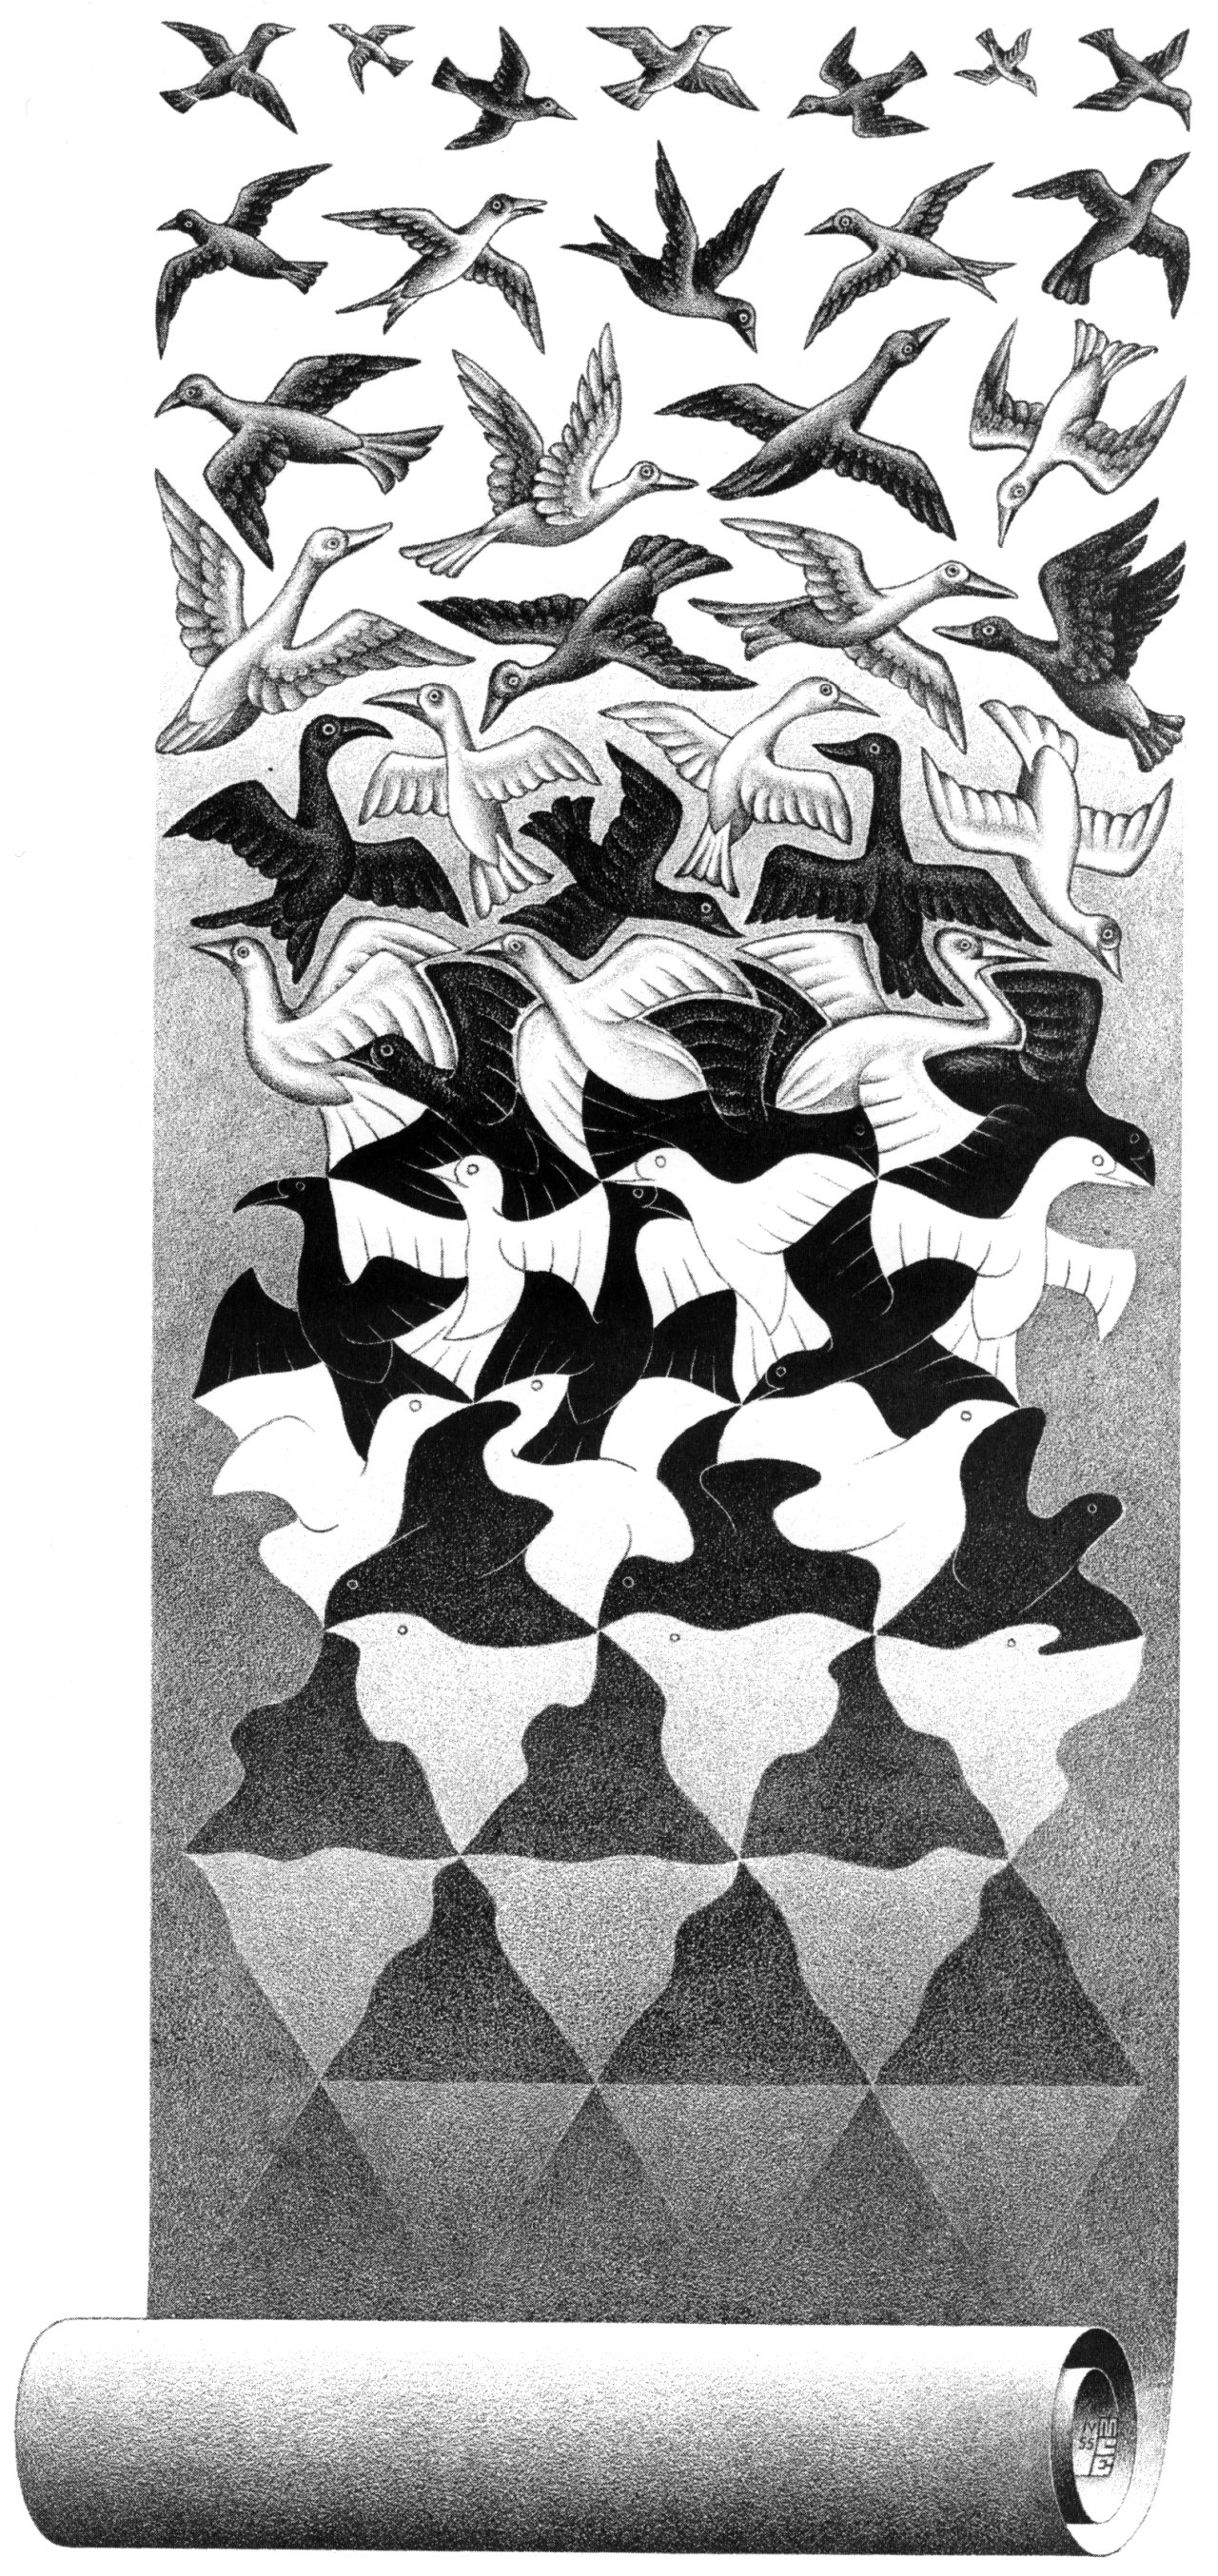
\includegraphics[scale=0.35]{img/Escher-Liberation-1955.eps}
 \captionsetup{labelformat=empty}
 \caption{Escher, Liberation, 1955}
 \label{fig:Escher-liberation}
\end{wrapfigure}

Humans gradually developed the habit of sorting things. The similar things are classified together. The methods and properties those applies to the entire class are also valid for every thing in that class. In this way, we needn't repeately solve the concrete individual problems one by one, but solve the abstract problems for a whole class. It greatly improved our ability to understand and master the world.

We generalized the abstract `folding' operation from sum and factorial for numbers. We observed their similar structures, abstract zero in sum, and one in factorial to unit element; then abstract the add in sum, and the multiplication in factorial to binary operation. As the result, we found the fold operation for numbers in a higher level. With this powerful tool, we then further solved a large sort of problems that are isomorphic to natural number, such as the Fibonacci numbers.

As another example, we also defined the abstract $foldr$ operation for list in chapter 1. With this tool, we can sum a list of numbers as $sum = foldr(0, +)$; we can also multiply them as $product = foldr(1, \times)$. In computer programming, there is a data structure called `binary search tree'. We introduced about binary tree in chapter 2. The binary search tree is a special binary tree that its elements are comparable\footnote{The meaning of comparable is abstract. If the elements are numbers, we can compare which one is bigger, if they are words, we can compare their lexicographical order.}. For any branch node, all elements in its left sub-trees are compared ahead of the element in this node; while all elements in its right sub-trees are compared behind it. Due to this kind of ordering, people also all it `sorted binary tree'. We can define insert operation for binary search tree as below:

\[
\begin{array}{rcl}
  insert(nil, x) & = & node(nil, x, nil) \\
  insert(node(l, y, r), x) & = & \left.
  \begin{cases}
  x < y\ : & node(insert(l, x), y, r) \\
  x > y\ : & node(l, y, insert(r, x))
  \end{cases} \right.
\end{array}
\label{eq:BST-insert}
\]

According to this definition, when insert element $x$ to binary search tree, if it is empty, the result is $node(nil, x, nil)$; otherwise, we need compare $x$ and the element $y$ in the branch node. If $x$ is ahead of $y$ (the `$<$' holds), then we recursively insert to the left sub-tree, else insert to the right sub-tree. Are there any similarity among the insert operation, sum, and factorial? Insertion is also binary operation, $nil$ can be considered as unit element. Then we can apply the abstract fold operation to turn a list of elements into a binary search tree:

\[
build = foldr(nil, insert)
\]

Figure \ref{fig:bst-example} shows the binary search tree generated when compute $build\ [4, 3, 1, 8, 2, 16, 10, 7, 14, 9]$.

\begin{figure}[htbp]
  \centering
  \includegraphics[scale=0.5]{img/bst-example.ps}
  \caption{The binary search tree generated from folding.}
  \label{fig:bst-example}
\end{figure}

We have similar experience when develop the concept of add. The initial addition is for specific things, like the fruits being collected, the prey being hunted. People later abstract the addition for numbers and remove the specific meanings for things. Then next we extended the understanding to numbers from integers to fractions. Although the detailed addition process is quite different, we need firstly unify the denominators, then add the nominators together, and finally reduce the fraction, people generalized the two different processes to the addition for rational numbers. We learned to think about the essence and principles of addition. Every time when people extend the concept of numbers, there is a new definition for addition. Along this way, we defined the addition for real numbers and complex numbers. We found the method established for abstract things without specific meanings has a greater scope of application. Abstract method can solve a whole kind of problems rather than the individual ones. Similar things happen in computer engineering, people developed the object-oriented method, generic type system, and dynamic type system, all these are sort of mechanisms to support abstraction.

We should always ask an important question when developing the abstract tools and generic methods. ``What is the applicable scope for the abstraction? When will the abstraction be invalid?'' It could lead to ridiculous result if ignore this. One example is about the sum of the infinite geometric series $1 + x + x^2 + x^3 + ... = 1/(1-x)$. It is so powerful that people can solved the Zeno's paradox\footnote{Here it is the Achilles and turtle paradox, which is one of the four famous paradoxes by Zeno, the ancient Greek philosopher. Achilles is a hero in ancient Greek. Zeno supposed Achilles wanted to catch up with the turtle ahead of him. When he ran to the position where the tortoise left, the tortoise had moved a short distance forward. Achilles must continue to run to that new position, but the turtle moved forward again. Repeated this process, Zeno argued that Achilles would never catch up the turtle. We'll explain Zeno's paradox in detail in Chapter 5.} with it. The mathematicians in the 17 Century substituted $x$ with -1, then got a result of $1 - 1 + 1 - 1 + ... = 1/2$. While, someone had a different idea that, $S = (1 - 1) + (1 - 1)+ ... = 0$. And there was even more different one: $S = 1 + (-1 + 1) + (-1 + 1) + ... = 1$. There were people supported the result should be 1/2, because $S = 1 - (1 - 1 + 1 - 1 + ...) = 1 -S$, solving this equation gave that $S = 1/2$. The Italian mathematician Grandi (1671 - 1742) found more surprised results. By using the infinite series:

\[
\def\arraystretch{2.2}
\begin{array}{l}
\dfrac{1}{1 + x + x^2} = 1 - x + x^3 - x^4 + x^6 - x^7 + ... \\%[5pt]
\dfrac{1}{1 + x + x^2 + x^3} = 1 - x + x^4 - x^5 + x^8 - x^9 + ... \\
...
\end{array}
\]

Let $x = 1$, Grandi found the sum of the infinite series $1 - 1 + 1 - 1 + 1 - 1 + ...$ could be 1/3, 4/1, ... Even the great mathematician Leibniz thought the result could be 0 or 1 with the same probability, therefore the `true' value should be the average 1/2. Grandi offered a new explanation that in 1710. Two brothers inherit a priceless gem from their father, whose will forbids them to sell it, so they agree that it will reside in each other's museums on alternating years. If this agreement lasts for all eternity between the brother's descendants, then the two families will each have half possession of the gem, even though it changes hands infinitely often\cite{HanXueTao16}. People kept suffering from these strange puzzles until the French mathematician Cauchy introduced the convergence concept for infinite series.

There are similar things in programming. When I implemented the natural merge sort algorithm \footnote{Natural merge sort is a sorting algorithm that permutes a list of elements in order. It firstly divides the elements into multiple groups, that every group contains the elements sorted. Then repeatedly merge these groups till all elements are ordered(\cite{LiuXinyu2017}, pp368).}, I need split the list into ordered groups, for example, split the list \texttt{[15, 9, 0, 12, 11, 7, 10, 5, 6, 13, 1, 4, 8, 3, 14, 2]} into groups of \texttt{[[15, 9, 0], [12, 11, 7], [10, 5], [6], [13, 1], [4], [8, 3], [14, 2]]}. The elements in the grouped sub-list are in descending order such as $15 > 9 > 0$. Then we can merge every two groups to get

\begin{verbatim}
[[15, 12, 11, 9, 7, 0], [10, 6, 5], [13, 4, 1], [14, 8, 3, 2]]
\end{verbatim}

Apply merge to every two groups again gives the next result

\begin{verbatim}
[[15, 12, 11, 10, 9, 7, 6, 5, 0], [14, 13, 8, 4, 3, 2, 1]]
\end{verbatim}

Then finally we can merge these two groups to get the sorted list:

\begin{verbatim}
[15, 14, 13, 12, 11, 10, 9, 8, 7, 6, 5, 4, 3, 2, 10]
\end{verbatim}

I found there is a pre-defined abstract grouping function \texttt{groupBy} in the library. It groups list with a given condition. For example \texttt{groupBy (==) "Mississippi"} gives result \texttt{["M", "i", "ss", "i", "ss", "i", "pp", "i"]}. Thus the same elements are grouped together. However, when I passed the `greater or equal' as the group condition, it generated the unexpected result. \texttt{groupBy (>=) [15, 9, 0, 12, 11, 7, 10, 5, 6, 13, 1, 4, 8, 3, 14, 2]} gives \texttt{[[15, 9, 0, 12, 11, 7, 10, 5, 6, 13, 1, 4, 8, 3, 14, 2]]}. This is because \texttt{groupBy} is realized with \texttt{span} like below:

\lstset{language=Haskell, frame=single}
\begin{lstlisting}
groupBy _  []      = []
groupBy eq (x:xs)  = (x:ys) : groupBy eq zs
    where (ys, zs) = span (eq x) xs

span _ []        = ([], [])
span p xs@(x:xs')
     | p x       = let (ys, zs) = span p xs' in (x:ys, zs)
     | otherwise = ([], xs)
\end{lstlisting}

For my example, \texttt{span} keeps checking if 15 is greater than the next element. As 15 is the biggest one in the list, therefore all the elements are grouped together. In fact, \texttt{groupBy} assumes the passed in group condition is the abstract `equality' condition, it must satisfy three properties: reflexivity, symmetry, and transitivity:

\begin{itemize}
\item reflexivity. $x = x$, any element equals to itself;
\item symmetry. if $x = y$, then $y = x$.
\item transitivity. if $x = y$, and $y = z$, then $x = z$. If two elements are identical, and one element equals to another, then the three elements are equal.
\end{itemize}

When use equality as condition to group the character list ``Mississippi'', all the three properties are satisfied, it generates the correct result. However, when pass the greater or equal ($geq$) as the abstract `equality' condition, it violates reflexivity and symmetry. That's the reason why it leads to the incorrect result.

This chapter introduces the basic abstract algebra structures. They are not only abstraction to numbers, but also the abstraction to concepts, properties, and relationships. They are the most valuable things from many great thoughts and minds. Some contents can challenge our limit of abstract thinking. It's quite common that you can't master them during the first time reading. I intended to add the stories about those great mathematicians, how they make breakthrough with unbelievable difficulties. I hope these interesting stories could encourage you keep going forward.

\section{Group}

\begin{wrapfigure}{R}{0.4\textwidth}
 \centering
 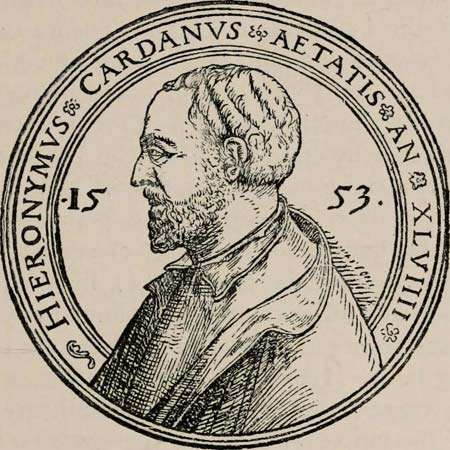
\includegraphics[scale=0.3]{img/Cardano.eps}
 \captionsetup{labelformat=empty}
 \caption{Gerolamo Cardano, 1501-1576}
 \label{fig:Cardano}
\end{wrapfigure}

\index{Gerolamo Cardano}
\index{Carl Friedrich Gauss}
\index{Fundamental theorem of algebra}

The group theory is originate from the history of equations. Equation is a powerful tool developed by ancient people. From the Rhind Mathematical Papyrus and Babylonian clay tablets, we know that the ancient Egyptians and ancient Babylonians mastered the method to solve the linear equation with one unknown and the quadratic equations. However, people didn't find the way to solve the generic cubic equations until the 16th Century. Several Italian mathematicians made great progress in solving cubic equations. Gerolamo Cardano finally published the radical solutions to generic cubic equation and quartic in his 1545 book {\em Ars Magna}. It does not only about to pursue higher and higher orders, but along with the totally new understanding about the numbers in the past thousand years. All the negative roots were discarded because we believed they were meaningless. People also thought the coefficients must be positive numbers. The equation $x^2 - 7x + 8 = 0$ is quite common today to us, but it had to be written in form of $x^2 + 8 = 7x$ to ensure the coefficients are positive. After Cardano list 20 different types of quartic equation in {\em Ars Magna}, he said there were another 67 types of quartic equation could not be given because the coefficient is either negative or zero\cite{HanXueTao2012}. It was the French mathematician François Viète who unified different forms of equations. Although most people thought the negative square root made no sense, Cardano found an interesting thing when solve the cubic equations like $x^3 = 15x +4$. His formula gives the intermediate result of $\sqrt[3]{2 + \sqrt{-121}} + \sqrt[3]{2 - \sqrt{-121}}$. Then it could next generate the three rational roots of 4, $-2 \pm \sqrt{3}$. Such problems expand our view to the irrational number, and finally, the great German mathematician Carl Friedrich Gauss developed the fundamental theorem of algebra\footnote{Gauss proved the fundamental theorem of algebra several times along his life. in 1799 at age of 22, he proved in his doctor thesis that every single-variable polynomial of degree $n$ with real coefficient has at least one complex root, thus deduced the single-variable equation of degree $n$ has and only has $n$ complex roots (counted with multiplicity for the same ones). Gauss gave another two different proofs in 1815 and 1816. In 1849, to celebrate the 50th anniversaries that Gauss received his doctor degree, he published the fourth proof and extend the coefficient to complex number.}.

\begin{figure}[htbp]
%\begin{wrapfigure}{R}{0.3\textwidth}
 \centering
 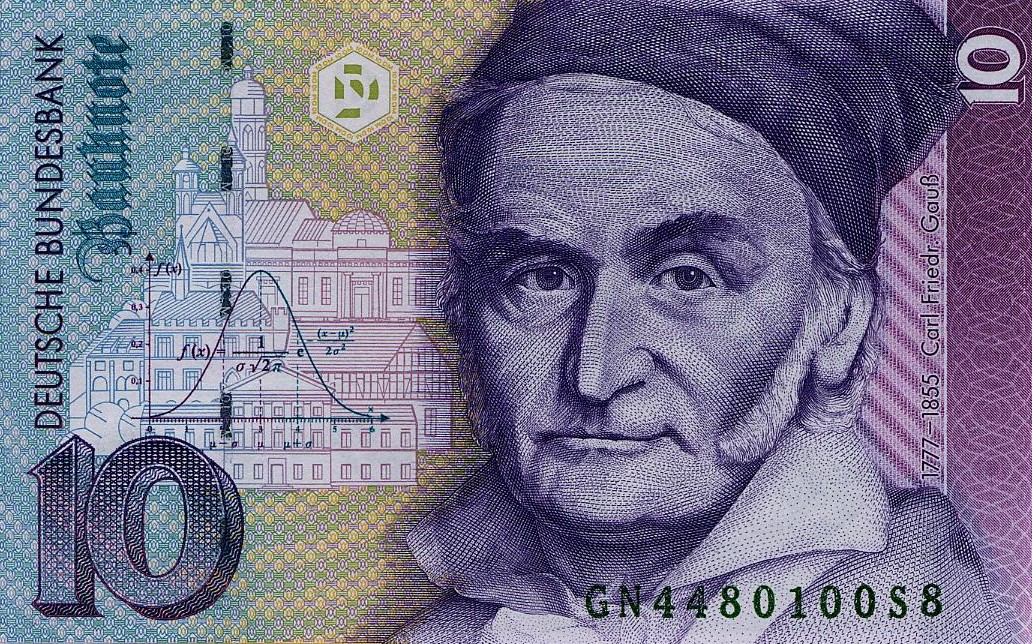
\includegraphics[scale=0.25]{img/Gaus.eps}
 \captionsetup{labelformat=empty}
 \caption{Gauss (1777-1855) in 10 Mark}
 \label{fig:Gauss}
%\end{wrapfigure}
\end{figure}

People encountered surprisingly difficulty when seek for radical solutions for generic quintic and higher order equations in the next 300 years. The breakthrough happened in the 19th Century with unexpected result. The French young Genius Évariste Galois developed a innovative idea, he was able to determine a necessary and sufficient condition for a polynomial to be savable by radicals while still in his teens\footnote{Around 1770, Joseph Louis Lagrange began the groundwork that unified the method to solve equations, he introduced the new idea to permute roots in the form of Lagrange resolvents. But he didn't consider the combination among the permutations. In 1799 The Italian mathematician Paolo Ruffini marked a major improvement, developing Lagrange's work on permutation theory. However, in general, Ruffini's proof was not considered convincing, and was discovered later incomplete. In 1824, the young Norwegian mathematician Niels Henrik Abel first completed proof demonstrating the impossibility of solving the general quintic equation in radicals. It is called `Abel–Ruffini theorem' nowadays. We know that there are radical solutions to the special quintic equation $x^5-1=0$. In what condition a polynomial is solvable in radicals? This problem was completely solved by Galois\cite{Wiki-Galois-theory}.}.

%\begin{figure}[htbp]
\begin{wrapfigure}{L}{0.4\textwidth}
 \centering
 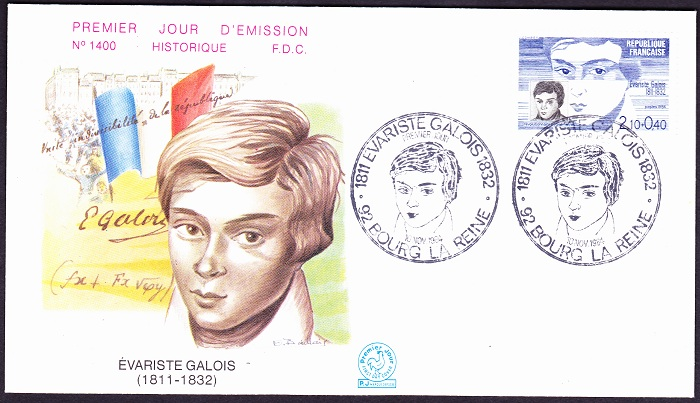
\includegraphics[scale=0.4]{img/galois.eps}
 \captionsetup{labelformat=empty}
 \caption{Galois, 1811 - 1832}
 \label{fig:Galois}
\end{wrapfigure}
%\end{figure}

\index{Galois}
It was a tragedy in Galois' short 20 years life, but his work laid the foundations of abstract algebra. Galois was born on 25 October 1811 in Paris. His mother, the daughter of a jurist, was a fluent reader of Latin and classical literature and was responsible for her son's education for his first twelve years. In 1823, he entered a prestigious school in Paris. At the age of 14, he began to take a serious interest in mathematics. He found a copy of {\em Elements} adapted by Legendre which, it is said, he read "like a novel" and mastered at the first reading. At 15, he was reading the original papers of Joseph-Louis Lagrange, which likely motivated his later work on equation theory, yet his classwork remained uninspired, and his teachers accused him of affecting ambition and originality in a negative way.

In 1828, he attempted the entrance examination for the École Polytechnique, the most prestigious institution for mathematics in France at the time, without the usual preparation in mathematics, and failed for lack of explanations on the oral examination. In that same year, he entered the École Normale, a far inferior institution for mathematical studies at that time, where he found some professors sympathetic to him.

In 1829 April, Galois' first paper, on continued fractions, was published. It was at around the same time that he began making fundamental discoveries in the theory of polynomial equations. He submitted two papers on this topic to the Academy of Sciences. But both were rejected due to some reasons\footnote{There was saying that the paper was lost by Cauchy. Actually, Cauchy refereed these papers, but refused to accept them for publication for reasons that still remain unclear. However, in spite of many claims to the contrary, it is widely held that Cauchy recognized the importance of Galois' work, and that he merely suggested combining the two papers into one in order to enter it in the competition for the Academy's Grand Prize in Mathematics. Cauchy, an eminent mathematician of the time, though with political views that were at the opposite end from Galois', considered Galois' work to be a likely winner\cite{Wiki-Galois}.}

On July 28 1829, Galois' father, a mayor of the village, committed suicide after a bitter political dispute with the village priest\cite{Wiki-Galois}. On August 3, Galois made his second and last attempt to enter the Polytechnique, and failed yet again. It is undisputed that Galois was more than qualified; however, accounts differ on why he failed. More plausible accounts state that Galois made too many logical leaps and baffled the incompetent examiner, which enraged Galois. Having been denied admission to the Polytechnique, Galois took the Baccalaureate examinations in order to enter the École Normale. He passed. His examiner in mathematics reported, ``This pupil is sometimes obscure in expressing his ideas, but he is intelligent and shows a remarkable spirit of research.''

\begin{figure}[htbp]
%\begin{wrapfigure}{L}{0.4\textwidth}
 \centering
 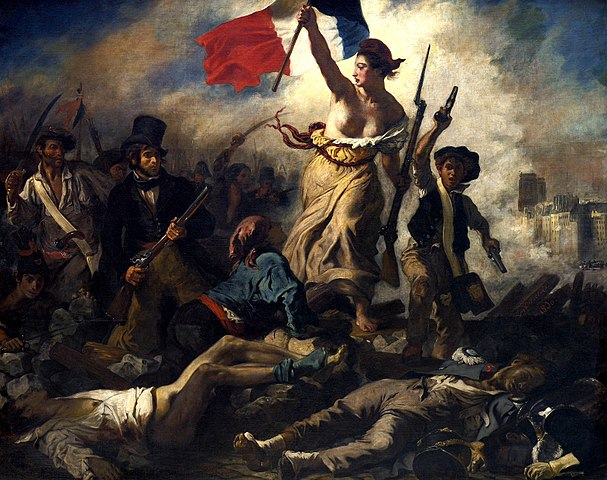
\includegraphics[scale=0.4]{img/lltp.jpg}
 \captionsetup{labelformat=empty}
 \caption{Eugène Delacroix, Liberty Leading the People, 1830, Louvre, Paris}
 \label{fig:Liberty-Leading-the-People}
%\end{wrapfigure}
\end{figure}

In February 1830, following Cauchy's suggestion Galois submitted his memoir on equation theory to the Academy's secretary Joseph Fourier, to be considered for the Grand Prix of the Academy. Unfortunately, Fourier died soon after, and the memoir was lost. The prize was awarded that year in June to Niels Henrik Abel\footnote{The young Norwegian mathematician Abel died on April 6, 1829. He made pioneering contributions in a variety of fields. His most famous single result is the first complete proof demonstrating the impossibility of solving the general quintic equation in radicals. He was also an innovator in the field of elliptic functions, discoverer of Abelian functions. He made his discoveries while living in poverty and died at the age of 26 from tuberculosis.} posthumously and also to Carl Gustav Jacob Jacobi\cite{HanXueTao2009}.

Galois lived during a time of political turmoil in France. The July Revolution broke out in France in 1830\footnote{The Bourbon monarch was restored after Napoleon's defect in Waterloo. King Charles X cleaned the soldiers who had worked for Napoleon in the army and caused dissatisfaction among the people. Continues with a series of failures in politics, economy, culture, religion, and diplomacy, Charles X signed the July Ordinances on July 25, 1830. These, among other steps, suspended the liberty of the press, dissolved the newly elected Chamber of Deputies, and excluded the commercial middle-class from future elections. It triggered the armed uprising of people, overthrew the Bourbon monarch through revolution. It ended with Louis-Philippe becoming king. Known as the July Monarchy.}. While their counterparts at the Polytechnique were making history in the streets, Galois and all the other students at the École Normale were locked in by the school's director. Galois was incensed and wrote a blistering letter criticizing the director, which he submitted to the Gazette des Écoles, signing the letter with his full name. Although the Gazette's editor omitted the signature for publication, Galois was expelled.

Galois quit school and joined the staunchly Republican artillery unit of the National Guard. He divided his time between his mathematical work and his political affiliations. Due to controversy surrounding the unit, soon after Galois became a member, on December 31, 1830, the artillery of the National Guard was disbanded out of fear that they might destabilize the government. He was arrested the on May 10, 1831, but was acquitted on June 15. On the Bastille Day (July 14), Galois was at the head of a protest, wearing the uniform of the disbanded artillery, and came heavily armed with several pistols, a rifle, and a dagger. He was again arrested. On 23 October, he was sentenced to six months in prison for illegally wearing a uniform. Early in 1831, Siméon Poisson asked him to submit his work on the theory of equations, which he did on January 17, 1831. Around July 4, 1831, Poisson declared Galois' work ``incomprehensible'', declaring that ``The argument is neither sufficiently clear nor sufficiently developed to allow us to judge its rigor\footnote{However, the rejection report ends on an encouraging note: ``We would then suggest that the author should publish the whole of his work in order to form a definitive opinion.''\cite{Wiki-Galois}}''. While Poisson's report was made before Galois' July 14 arrest, it took until October to reach Galois in prison. It is unsurprising, in the light of his character and situation at the time, that Galois reacted violently to the rejection letter, and decided to abandon publishing his papers through the Academy and instead publish them privately through his friend Auguste Chevalier. Apparently, however, Galois did not ignore Poisson's advice, as he began collecting all his mathematical manuscripts while still in prison, and continued polishing his ideas until his release on April 29, 1832.

Shortly after released from prison, Galois was involved in a obscure duel because of love. On May 29, Galois was so convinced of his impending death that he stayed up all night writing letters to his friends and composing what would become his mathematical testament, the famous letter to Auguste Chevalier outlining his ideas, and three attached manuscripts.German mathematician Hermann Weyl said of this testament, ``This letter, if judged by the novelty and profundity of ideas it contains, is perhaps the most substantial piece of writing in the whole literature of mankind.'' In these final papers, he outlined the rough edges of some work he had been doing in analysis and annotated a copy of the manuscript submitted to the Academy and other papers.

When read Galois' 7 pages testament, there are some words really sad: ``these subjects are not the only ones that I have explored... But I don't have time, and my ideas are not yet well developed in this area, which is immense...it would not be too much in my interest to make mistakes so that one suspects me of having announced theorems of which I would not have a complete proof.'' The most impressed and saddest words are: ``I don't have time'' At the end of the letter, he asked his friend to ``Ask Jacobi or Gauss publicly to give their opinion, not as to the truth, but as to the importance of these theorems. Later there will be, I hope, some people who will find it to their advantage to decipher all this mess.''\cite{Galois-1832}

\begin{figure}[htbp]
%\begin{wrapfigure}{L}{0.4\textwidth}
 \centering
 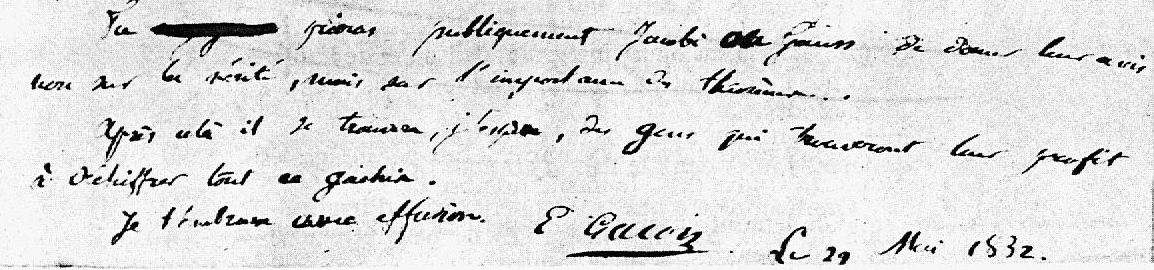
\includegraphics[scale=0.3]{img/GalSign.eps}
 \captionsetup{labelformat=empty}
 \caption{``E. Galois, le 29 mai 1832'' at the bottom of the last page in his testament.}
 \label{fig:GalSign}
%\end{wrapfigure}
\end{figure}

Early in the morning of May 30, 1832, Galois was injured badly in the duel. He was shot in the abdomen. A passing farmer found him, and sent Galois to the hospital. He died the following morning at ten o'clock, after refusing the offices of a priest. His younger brother was notified, and came to the hospital. His last words to his brother Alfred were: ``Don't cry, Alfred! I need all my courage to die at twenty!'' We don't know the exact reason behind the duel, whether it was a love tragedy or a political murder. Whatever the reason, a great talent mathematician was killed at the age of 20. He had only been studied mathematics for 5 years. Within the only 67 pages of Galois' collected works are many important ideas that have had far-reaching consequences for nearly all branches of mathematics.

Chevalier and Galois' young brother published the testament in {\em Revue encyclopedique}, but it was not noticed. It might be too brief and hard, there was almost no any impact to the mathematics in that years\footnote{The similar lessons happened to Abel as well. When he use his own money to published the paper about why quintic equation couldn't be solved by radicals in 1824, to save money, he tried all means to consolidate the paper in 6 pages. As the result, it's too brief and obscure for people to notice and understand it till Abel's death.}. Decades passed, in 1843 Liouville reviewed Galois manuscript and declared it sound. It was finally published in the October–November 1846 issue of the {\em Journal de Mathématiques Pures et Appliquées}. The most famous contribution of this manuscript was a novel proof that there is no quintic formula – that is, that fifth and higher degree equations are not generally solvable by radicals. Although Abel had already proved the impossibility of a "quintic formula" by radicals in 1824, Galois' methods led to deeper research in what is now called Galois theory. For example, one can use it to determine, for any polynomial equation, whether it has a solution by radicals. Liouville thought about this tragedy and commented it in the introduction to Galois' paper: ``Perhaps, his exaggerated desire for conciseness was the cause of this defect, and is something which one must endeavor to refrain from when dealing with the abstract and mysterious matters of pure Algebra. Clarity is, indeed, all the more necessary when one has intention of leading the reader away from the beaten roads into the desert... But at present all that has changed. Alas, Galois is no more! Let us cease carrying on with useless criticisms; let us leave its defects, and instead see its qualities... My zeal was soon rewarded. I experienced great pleasure the moment when, after having filled in the minor gaps, I recognized both the scope and precision of the method that Galois proved.''\cite{Liouville-1846}

In 1870, French mathematician Camille Jordan wrote the book {\em Traité des substitutions et des équations algébriques} based on Galois' theory\footnote{Galois' theory was notoriously difficult for his contemporaries to understand, especially to the level where they could expand on it. For example, in his 1846 commentary, Liouville completely missed the group-theoretic core of Galois' method. Joseph Alfred Serret who attended some of Liouville's talks, included Galois' theory in his 1866 (third edition) of his textbook Cours d'algèbre supérieure. Jordan was Serret's pupil. Outside France, Galois' theory remained more obscure for a longer period. It turned a century in Britain. In Germany, it was Dedekind lectured on Galois' theory at Göttingen in 1858, showing a very good understanding.}. Galois' most significant contribution to mathematics is his development of Galois theory. He realized that the algebraic solution to a polynomial equation is related to the structure of a group of permutations associated with the roots of the polynomial, the Galois group of the polynomial. It laid the foundation of group theory and lead to the development of abstract algebra and modern mathematics. As the ironic result ``Instead of the political revolution, what Galois actually triggered was the mathematics revolution\cite{StepanovRose15}.''

\subsection{Group}
\index{Group}

Let us start the journey from groups to understand what Galois landed for abstract algebra.

\begin{definition} A group is a set $G$ equipped with a binary operation ``$\cdot$'', which satisfied four axioms:

\begin{enumerate}
\item \textbf{Closure}: For all $a, b \in G$, the result of the operation $a \cdot b \in G$;
\item \textbf{Associativity}: For all $a, b, c$ in $G$, $(a \cdot b) \cdot c = a \cdot (b \cdot c)$;
\item \textbf{Identity element}: There exists an element $e$ in $G$ such that, for every element $a$ in G, the equation $a \cdot e = e \cdot a = a$ holds;
\item \textbf{Inverse element}: For each element $a \in G$, there exists an element $a^{-1}$, such that $a \cdot a^{-1} = a^{-1} \cdot a = e$, where $e$ is the identity element.
\end{enumerate}
\end{definition}

The binary operation is often called ``multiplication'', and the ``product'' $a \cdot b$ is usually written as $ab$. $e$ is the identity element. The number of elements in a group can be finite or infinite, thus the group is called finite group or infinite group. the \textbf{order} of a finite group is the number of the elements in the group. A group contains infinite many elements is said to have infinite order.

The ``multiplication'' operation of the group may not be commutative like the normal multiplication for numbers. For example, all the invertible matrix with real entities, together with the matrix multiplication form a group. However, the matrix multiplication order matters, it is not commutative. Groups for which the community equation $ab = ba$ always holds are called \textbf{abelian} groups (in honor of Abel).

To help understanding the definition of group, let us see some examples.

\begin{enumerate}
\item 整数加法群:群元素是全体整数,二元运算是加法。简称为整数加群;
\item 所有整数除以5的余数构成的集合,也就是$\{0, 1, 2, 3, 4\}$。二元运算是相加后再除以5取余数。例如$3 + 4 = 7 \bmod 5 = 2$。这样构成的群称为整数模5加法群,记为$Z_5$。通过取余数对整数进行分类叫做模$n$剩余类;
\item 转动魔方所形成的群:群元素是各种魔方转动的方式\footnote{魔方的旋转方式共有18种。可以沿着正面、反面、顶面、底面、左面、右面旋转,分别用字母$F$、$B$、$T$、$D$、$L$、$R$代表,每面可以旋转90度、180度、-90度。例如左面旋转90度、180度、-90度分别可以记为:$L$、$L^2$、$L'$\cite{Wiki-Rubik-Cube-group}。再加上恒等变换,一共19个元素。},二元运算是先进行某种转动后再进行另一种转动。这种运算常被称作转动的合成;

\begin{figure}[htbp]
%\begin{wrapfigure}{L}{0.4\textwidth}
 \centering
 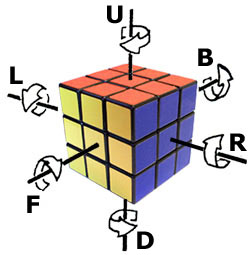
\includegraphics[scale=0.8]{img/Rubik_cube_notation.eps}
 %\captionsetup{labelformat=empty}
 \caption{魔方六个面共有18种转动方式,再加上恒等变换。这些转动方式在合成下构成一个群。}
 \label{fig:Rubik-cube-notation}
%\end{wrapfigure}
\end{figure}

\item 平面绕某点的所有旋转构成一个群。群元素是所有的旋转角度,二元运算是先旋转某一角度,然后再旋转另一角度。
\end{enumerate}

而下面这些不是群:

\begin{enumerate}
\item 所有不等于零的整数和乘法不构成群,我们不能规定单位元为1,因为3没有逆元(1/3不是整数);
\item 同理,模5的余数集合$\{0, 1, 2, 3, 4\}$和模5的乘法不构成一个群,但如果把5的整倍数去掉,则集合$\{1, 2, 3, 4\}$和模5的乘法构成一个群。可以从下面的“乘法表”看出来:

  \begin{tabular}{c|cccc}
    & 1 & 2 & 3 & 4 \\
  \hline
  1 & \textbf{1} & 2 & 3 & 4 \\
  2 & 2 & 4 & \textbf{1} & 3 \\
  3 & 3 & \textbf{1} & 4 & 2 \\
  4 & 4 & 3 & 2 & \textbf{1}
  \end{tabular}

因此,单位元是1,它的逆元是其本身;2和3互为逆元,4的逆元还是4;
\item 虽然模5的非零余数在模乘法下构成一个群,但是模4的非零余数在模乘下却不构成群。观察模4的乘法表:

  \begin{tabular}{c|cccc}
    & 1 & 2 & 3 \\
  \hline
  1 & 1 & 2 & 3 \\
  2 & 2 & \textbf{0} & 2 \\
  3 & 3 & 2 & 1 \\
  \end{tabular}

注意到$(2 \times 2) \bmod 4 = 0$,不在集合$\{1, 2, 3\}$中。这个反例告诉我们,只有和$n$互素的余数集合,在模$n$乘法下才能构成群,这种群称为整数模$n$乘法群。自然,如果$p$是素数,则$\{1, 2, ..., p-1\}$构成模$p$乘法群。
\item 全体有理数在乘法下不构成一个群。尽管任何形如$p/q$的有理数都有逆元$q/p$,但是0没有逆元。所有非零有理数在乘法下才构成一个群。
\end{enumerate}

\begin{Exercise}
\Question{全体偶数在加法下是否构成一个群?}
\Question{能否找到一个整数的子集,使得它在整数乘法下构成一个群?}
\Question{所有正实数在乘法下是否构成一个群?}
\Question{整数在减法下是否构成一个群?}
\Question{举一个只有两个元素的群的例子。}
\Question{魔方群的单位元是什么?$F$的逆元是什么?}
\end{Exercise}

\subsection{幺半群与半群}
群的限制条件比较严格,从上一节的反例中,我们看到有一些常用的代数结构无法满足群的全部条件。有时我们并不需要一定能够取逆元,如果放宽条件,就可以得到幺半群(monoid)这种结构。

\index{幺半群(monoid)}
\begin{definition}
\textbf{幺半群}是一个集合$S$和其上定义的二元运算$\cdot$,它们遵循两条公理:
\begin{enumerate}
\item 结合性公理:$S$中和任何三个元素满足$(a \cdot b) \cdot c = a \cdot (b \cdot c)$;
\item 单位元公理:$S$中存在一个元素$e$,使得对任何$a \cdot e = e \cdot a = e$。
\end{enumerate}
\end{definition}

可以看到幺半群与群的定义类似,只是去掉了取逆运算的消去公理。可以立即看到,上一节群的反例中有不少是幺半群,例如整数乘法构成幺半群,单位元是1。幺半群在编程中很常见。我们在下一章介绍范畴论时还会再仔细介绍幺半群这一特别重要的结构。下面是一些幺半群的例子:

\begin{enumerate}
\item 给定字符集后,长度有限的字符串在拼接操作下构成幺半群。幺半群的元素是字符串,二元运算是拼接操作。单位元是空串。
\item 由字符串推广到列表(List A),在连接操作下构成幺半群。幺半群的元素是列表,二元运算是连接操作($\doubleplus$)。单位元是空列表nil。

为此,我们可以写出以下的程序,用幺半群来定义字符串和列表的代数结构。

\begin{lstlisting}
instance Monoid (List A) where
    e = nil
    (*) = (++)
\end{lstlisting}

这样针对字符串和列表的的“叠加”操作,完全可以将抽象程度提升到幺半群上来\footnote{我们将在下一章讲解范畴论时介绍如何实现这样的抽象叠加操作}。例如下面的“合并”操作定义对任何幺半群都有效:

\[
concat = foldr\ e\ (*)
\]

这样就可以用$concat$合并列表,如

$concat\ [[1], [2], [3], [1, 2], [1, 3], [2, 3], [1, 2, 3], [1, 3, 2]]$的结果是[1, 2, 3, 1, 2, 1, 3, 2, 3, 1, 2, 3, 1, 3, 2]。

\index{堆(heap)}
\index{斜堆(skew heap)}
\item 堆(heap)是编程中一种常见的数据结构,堆顶元素总是最小的堆称为最小堆(或小顶堆、小根堆)。有一种“斜堆”(skew heap)可以用上一章定义的二叉树来实现(\cite{LiuXinyu2017}第7.3节):

\begin{lstlisting}
data SHeap A = nil | node (SHeap A, A, SHeap A)
\end{lstlisting}

可以看出,除了名称,斜堆的定义和二叉树完全一样。非空堆的最小元素在树的根节点中。定义斜堆的“归并”(merge)运算如下:

\[
\begin{array}{rcl}
merge(nil, h) & = & h \\
merge(h, nil) & = & h \\
merge(h_1, h_2) & = &
  \begin{cases}
  k_1 < k_2 : & node(merge(r_1, h_2), k_1, l_1) \\
  \text{否则}: & node(merge(h_1, r_2), k_2, l_2)
  \end{cases}
\end{array}
\]

如果其中任一堆为空,则归并结果为另一个堆。非空情况下,$h_1$和$h_2$分别可以表示为 $node(l_1, k_1, r_1)$ 和 $node(l_2, k_2, r_2)$。我们比较根节点,选择较小的作为新的根。然后把含有较大元素的树合并到某一子树上。最后再把左右子树交换。若$k_1 < k_2$,选择$k_1$作为新的根。我们既可以将$h_2$和$l_1$合并,也可以将$h_2$和$r_1$合并。不失一般性,我们合并到$r_1$上。然后交换左右子树,最后的结果为$(k_1, merge(r_1, h_2), l_1)$。注意这个归并的二元运算是递归的。这样所有斜堆组成的集合,在这一归并运算下构成一个幺半群。单位元是空堆nil。

\index{配对堆(pairing heap)}
\item 堆也可以用上一章介绍的多叉树实现。有一种堆叫做配对堆(pairing heap)它的定义如下(\cite{LiuXinyu2017}第9.4节):

\begin{lstlisting}
data PHeap A = nil | node (A, List (PHeap A))
\end{lstlisting}

除了名称外,这个定义和上一章的多叉树的结构完全相同。这是一个递归定义,一个配对堆要么为空,要么是一棵多叉树,包含一个根节点和一组子树。非空堆的最小元素在多叉树的根节点中。我们可以定义配对堆的归并操作:

\[
\begin{array}{rcl}
merge(nil, h) & = & h \\
merge(h, nil) & = & h \\
merge(h_1, h_2) & = &
  \begin{cases}
  k_1 < k_2 : & node(k_1, h_2 : ts_1)) \\
  \text{否则} : & node(k_2, h_1 : ts_2)) \\
  \end{cases}
\end{array}
\]

如果任一堆为空,则归并结果为另一个堆。非空情况下,两个堆$h_1$和$h_2$分别可以表示为 $node(k_1, ts_1)$ 和 $node(k_2, ts_2)$。我们比较两个堆的根节点元素,令根节点较大的一个作为另一个的新子树。这样所有的配对堆组成的集合,在归并操作下构成一个幺半群,单位元是空堆nil。

\end{enumerate}

\index{半群(semigroup)}
如果再进一步把单位元的限制也去掉,我们就得到了半群(semigroup)这种代数结构。

\begin{definition}
半群是一个集合和定义在其上的可结合的二元运算。
\end{definition}

半群的二元运算是可结合的,所以满足结合律:半群中的任何三个元素$a$、$b$、$c$满足$(ab)c = a(bc)$。半群的条件更为宽松,下面是一些半群的例子:

\begin{enumerate}
\item 全体正整数构成的加法半群、乘法半群;
\item 全体偶数构成的加法半群、乘法半群。
\end{enumerate}

如前所述,人们常将定义在群、幺半群、半群上的二元运算叫做“乘法”,因此我们可以用“乘方”来表示连续的二元运算。如:$x \cdot x \cdot x = x^3$。一般地,群和幺半群的“幂”可以递归地定义如下:

\[
x^n = \left .
  \begin{cases}
  n = 0 : & e \\
  \text{其它}: & x \cdot x^{n-1}
  \end{cases}
\right .
\]

但是半群没有单位元,所以$n$必须是非零正整数:

\[
x^n = \left .
  \begin{cases}
  n = 1 : & x \\
  \text{其它}: & x \cdot x^{n-1}
  \end{cases}
\right .
\]

\begin{Exercise}
\Question{布尔值构成的集合\{True, False\},在“逻辑或”运算$\lor$下构成一个幺半群。称为任意(Any)逻辑幺半群。它的单位元是什么?}
\Question{布尔值构成的集合\{True, False\},在“逻辑与”运算$\land$下构成一个幺半群。称为全部(All)逻辑幺半群。它的单位元是什么?}
\Question{对可比类型的元素进行比较时,会有三种结果,我们把它们抽象为$\{<, =, >\}$\footnote{一些编程语言,如C、C++、Java用负数、零、正数表示这三种关系。Haskell中用GT, EQ, LE表示。},针对这个集合,定义一个二元运算使得它们构成一个幺半群。这个幺半群的单位元是什么?}
\Question{证明群、幺半群、半群的幂满足交换律:$x^mx^n = x^nx^m$}
\end{Exercise}

\subsection{群的性质}

抽象代数最强大的思想在于我们可以不关心抽象概念所代表的实际物体的含义,而研究抽象结构间内在的规律。这些规律对所有被抽象的物体都适用。如果我们了解了一般群的内在规律,而群元素代表几何的点、线、面,则我们就获得了几何的规律;如果群元素是魔方的旋转,我们就获得了魔方变换的规律;如果群元素是编程中的某种数据结构,我们就得到了这种数据结构上的算法。我们这一节介绍一些群上的重要性质。

\begin{theorem}
群的单位元是唯一的。
\end{theorem}

\begin{proof}
假设存在另一单位元$e'$,使得对任意元素$a$满足$e'a = ae' = a$。我们有$e = ee'= e'$。这样就证明了单位元的唯一性。
\end{proof}

不仅群的单位元是唯一存在的,而且每个元素的逆也是唯一存在的。我们有下面的定理。

\begin{theorem}
逆元唯一存在。对群中的任意元素$a$,都存在且仅存在一个$a^{-1}$使得$aa^{-1} = a^{-1}a = e$。我们称$a^{-1}$为$a$的逆元。
\end{theorem}

\begin{proof}
根据群的消去公理,我们知道逆元存在。所以我们只需要证明逆元唯一。假设存在另一元素$b$,也满足$ab = ba = e$,我们在等式右侧“乘以”$a^{-1}$得:
\[
\begin{array}{rll}
aba^{-1} & = baa^{-1} = ea^{-1} & \\
& \Rightarrow be = a^{-1} & \text{对第二项用结合律} \\
& \Rightarrow b = a^{-1} & \text{逆元唯一}
\end{array}
\]
\end{proof}

\begin{figure}[htbp]
%\begin{wrapfigure}{L}{0.4\textwidth}
 \centering
 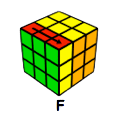
\includegraphics[scale=1.0]{img/Rubik-cube-F.eps}
 %\captionsetup{labelformat=empty}
 \caption{魔方的F变换,连续转动4次回到原位。}
 \label{fig:Rubik-cube-F}
%\end{wrapfigure}
\end{figure}

\index{群元素的阶}
我们在前面定义了群的阶,群的元素也可以定义阶。对群中的一个元$a$,能够满足$a^m = e$的最小正整数$m$叫做$a$的阶。如果这样的$m$不存在,我们说$a$的阶是无限的。例如前面例子中魔方旋转群中,$F$旋转4次就回到了原位,所以$F$的阶是4,而$F'$旋转两次回到原位,所以它的阶是2。再比如整数模5的乘法群,除了1以外,其他元素的4次幂都模5余1,所以他们的阶都是4。我们有如下有趣的定理。

\begin{theorem}
有限群的每个元素都有有限的阶。
\end{theorem}

\begin{proof}
如果有限群$G$的阶是$n$,对任意元素$a$,构造集合$\{a, a^2, ..., a^{n+1}\}$。这个集合有$n+1$个元,但是群的阶是$n$,所以根据鸽笼原理,一定有两个元素是相等的, 不妨记这两个元素为$a^i$和$a^j$,其中$0 < i < j \leq n + 1$。我们有:
\[
\begin{array}{rcll}
a^ja^{-i} & = & a^{-i}a{i} & \text{由} a^i = a^j \\
a^ja^{-i} & = & e & \text{$a^i$和$a^{-i}$互为逆元} \\
a^{j-i} & = & e & a\text{的阶为} j - i
\end{array}
\]
所以$a$的阶为$j-i$是有限的。
\end{proof}

在第一章,我们比较随意地使用了“同构”一词来形容具有相同内在结构的事物。现在我们可以给出同态和同构的概念了。假设存在从某个集合$A$到另一个集合$B$的映射$f$。$a$和$b$是$A$中的两个元,$f(a)$和$f(b)$是它们在$B$中的像。我们考虑$A$上的二元封闭运算产生的元$a \cdot b$,在映射下在$B$中的像$f(a \cdot b)$。如果对$B$上的二元封闭运算总有

\[
f(a) \cdot f(b) = f(a \cdot b)
\]

\begin{figure}[htbp]
\centering
\begin{tikzpicture}[scale=0.8]
\draw (0, 0) circle[x radius=1cm, y radius=3cm]
      (5, 0) circle[x radius=1cm, y radius=3cm];
\path (0, 3) node[above] {$A$:自然数乘法半群}
      (5, 3) node[above] {$B$:平方数乘法半群};
\path (0, 0) node (b) {}
      (5, 0) node (fb) {}
      (0, 1.5) node (a) {}
      (5, 1.5) node (fa) {}
      (0, -1.5) node (c) {}
      (5, -1.5) node (fc) {};
\filldraw (0, 0) circle (1pt) node[above] {$b$}
      (5, 0) circle (1pt) node[above] {$f(b)$}
      (0, 1.5) circle (1pt) node[above] {$a$}
      (5, 1.5) circle (1pt) node[above] {$f(a)$}
      (0, -1.5) circle (1pt) node[above] {$ab$}
      (5, -1.5) circle (1pt) node[above] {$f(ab)$};
\draw[dashed, ->] (b) to node [above] {$f: x \to x^2$} (fb)
      (a) to [bend left] (fa)
      (c) to [bend right] (fc);
\end{tikzpicture}
\[
\begin{array}{rl}
a = 2 & f(a) = 4 \\
b = 3 & f(b) = 9 \\
ab = 6 & f(ab) = f(a)f(b) = 36
\end{array}
\]
\caption{同构}
\label{fig:isomorphism}
\end{figure}

\index{同态映射(homomorphism)}
我们就说$f$是从$A$到$B$的\textbf{同态映射}(homomorphism)。如果$f$是满射(surjection,即$B$中所有元素都在$A$中有原像),则称为同态满射。举一个例子,考虑一个奇偶判定函数$odd: Z \to Bool$,它接受一个整数,如果是奇数就返回真值True,否则返回假False。整数在加法下构成一个群。而布尔集合$\{True, False\}$在逻辑异或运算下也构成一个群。我们可以很容易验证:

\begin{enumerate}
\item $a$和$b$都是奇数,$odd(a)$和$odd(b)$都为真。它们的和是偶数,$odd(a+b)$为假。满足$odd(a) \oplus odd(b) = odd(a+b)$;
\item $a$和$b$都是偶数,$odd(a)$和$odd(b)$都为假。它们的和也是偶数,$odd(a+b)$也为假。满足$odd(a) \oplus odd(b) = odd(a+b)$;
\item $a$和$b$一奇一偶,$odd(a)$和$odd(b)$一真一假。它们的和为奇数,$odd(a+b)$为真。满足$odd(a) \oplus odd(b) = odd(a+b)$;
\end{enumerate}

\index{同构(isomorphism)}
\index{自同构(automorphism)}
如果$f$不仅是满射,还是单射(injection)。那么它就是一一映射。这种情况下,我们称$f$是从$A$到$B$的同构映射,简称\textbf{同构}(isomorphism)。记为$A \cong B$。同构是一种非常强大的关系,不仅两个群可以同构,半群、幺半群以及其他代数结构也可以同构,如图\ref{fig:isomorphism}所示。如果$A$和$B$同构,那么抽象地来看,它们没有什么区别,只有命名上的不同。如果$A$上有一个代数性质,那么在$B$上也有一个完全类似的性质\cite{ZhangHeRui1978}(25页)。另外,$A$与$A$之间的同构映射称为$A$的\textbf{自同构}(automorphism)。例如整数加群在取相反数下成为自同构。

\begin{figure}[htbp]
\centering
\begin{tikzpicture}
\path (0, 0) node[below] {猫}
      (0, 2) node[above] {羊}
      (-2, 2) node[above] {狗}
      (-2, 0) node[below] {牛};
\filldraw (0, 0) circle (4pt) node (cat) {} --
   (0, 2) circle (4pt) node (sheep) {} --
   (-2, 2) circle (4pt) node (dog) {} --
   (-2, 0) circle (4pt) node (cow) {};
\draw (dog) -- (cat) -- (cow);

\filldraw[fill=gray, draw=black, pattern=north west lines]
    (3, 0) circle (4pt) node (collar) {} --
    (5.6, 0) circle (4pt) node (bell) {} --
    (4.3, 2.3) circle (4pt) node (milk) {} -- (collar) --
    (4.3, 1) circle (4pt) node (wool) {} -- (bell);
\path (3, 0) node[below] {项圈}
      (5.6, 0) node[below] {铃铛}
      (4.3, 2.3) node[above] {奶}
      (4.3, 1) node[below] {毛};

\draw[dashed, ->] (dog) .. controls (-2.5, 1.5) .. (collar)
    (sheep) to[bend left] (wool)
    (cat) to[bend right] (bell)
    (cow) .. controls (-3, 3) ..(milk);
\end{tikzpicture}
\[
\begin{array}{rl}
f(狗) = 项圈 & f(猫) = 铃铛 \\
f(羊) = 毛 & f(牛) = 奶
\end{array}
\]
\caption{图的同构(graph isomorphsim)具有不同的定义。它反映了看似不同的两个图,具有相同的结构。}
\label{fig:graph-isomorphism}
\end{figure}

面对群这种抽象的代数结构时,具体的例子可以帮助我们理解。我们会不自觉地选出一个自己熟悉的代表,例如整数加群,然后看看各种概念,性质在其上是怎样的。但有时这容易形成一种错觉。感觉群的元素大多是一些实体,例如各种数;并且二元运算大多像普通加法、乘法那样可以交换。我们接下来介绍的“变换群”是一个例外,一方面,它不是阿贝尔群,运算不可交换;另一方面群元素不是数,而是变换。

所谓变换,就是一个集合$A$到$A$自身的映射。记为$\tau : A \to A$。它把集合$A$的元素$a$映射为$\tau(a)$,即$a \to \tau(a)$。一个集合可以有多个不同的变换,例如下面是布尔集合的全部变换,我们记真为$T$、假为$F$。

\[
\begin{array}{rll}
\tau_1 : & T \to T, & F \to T \\
\tau_2 : & T \to F, & F \to F \\
\tau_3 : & T \to T, & F \to F \\
\tau_4 : & T \to F, & F \to T
\end{array}
\]

其中变换$\tau_3$和$\tau_4$是一一变换。针对一个集合$A$,我们将它的全体变换放到一起构成一个新的集合:

\[
S = \{\tau, \lambda, \mu, ...\}
\]

现在我们要规定一个S的二元代数运算,把它叫做乘法。为了方便起见,我们将$\tau(a)$用另一个符号表达:

\[
\tau: a \to a^\tau = \tau(a)
\]

这里$a^\tau$不是$a$的$\tau$次方的意思,它只是一个符号记法,表示变换的意思。我们观察$S$的两个元$\tau$和$\lambda$,

\[
\tau: a \to a^\tau,  \lambda: a \to a^\lambda
\]

那么$a \to (a^\tau)^\lambda = \lambda(\tau(a))$显然也是$A$的一个变换,现在我们规定把这个变换叫做$\tau$和$\lambda$的乘积。

\[
\tau\lambda: a \to (a^\tau)^\lambda = a^{\tau\lambda}
\]

读着不妨从前面布尔变换的集合里取几个变换来计算它们的乘积,不难验证这一乘法适合结合律,因为:

\[
\begin{array}{rl}
\tau(\lambda\mu): & a \to (a^\tau)^{\lambda\mu} = ((a^\tau)^\lambda)^\mu \\
(\tau\lambda)\mu: & a \to (a^{\tau\lambda})^\mu = ((a^\tau)^\lambda)^\mu
\end{array}
\]

现在不难看出当初我们选择乘方符号来表达变换的好处了。选择一套强大的符号系统是多年来数学发展的传统和法宝。欧拉、莱布尼茨都是选择和使用符号的大师。对这个乘法来说,$S$的单位元就是$A$的恒等变换$\epsilon: a \to a$。不难验证:

\[
\begin{array}{rl}
\epsilon\tau: & a \to (a^\epsilon)^\tau = a^\tau \\
\tau\epsilon: & a \to (a^\tau)^\epsilon = a^\tau
\end{array}
\]

所以$\epsilon\tau = \tau\epsilon = \tau$。这样$S$对这个乘法来说差不多已经构成一个群了。可惜,虽然说是差不多,到底还是差一点。因为任意变换$\tau$不一定有逆元。例如布尔变换集合中的$\tau_1$,它把任何布尔值都变换成真,不管用这4个变换中的哪一个,都无法把$\tau_1$变换回去。所以$\tau_1$没有逆元。

虽然$S$无法构成群,但是峰回路转,是它的一个子集$G$却有可能构成群。事实上,如果$G$只包含$A$的一一变换,则它在这个乘法下构成群。

\index{变换群(transform group)}
我们称,一个集合$A$的若干个一一变换对于上述规定的乘法所作成的群叫做$A$的一个\textbf{变换群}(transform group)。并且我们有以下重要的定理:

\begin{theorem}
一个集合$A$的所有一一变换构成一个变换群$G$。
\end{theorem}

变换群一般不是交换群(阿贝尔群),我们可以很容易地找到反例。考虑$\tau_1$是平面上的平移,它把原点(0, 0)移动到(1, 0),变换$\tau_2$是绕原点旋转$\pi/2$,但是:

\[
\begin{array}{rl}
\tau_1\tau_2: & (0, 0) \to (0, 1) \\
\tau_2\tau_1: & (0, 0) \to (1, 0)
\end{array}
\]

\begin{figure}[htbp]
\centering
\begin{tikzpicture}[scale=1]
\draw[->] (-0.5, 0) -- (2, 0) node[right] (x axis) {$x$};
\draw[->] (0, -1.5) -- (0, 1.5) node[above] (y axis) {$y$};
\path (0, -1) node[left] {$a$}
      (1, -1) node[right] {$b$}
      (1, 1) node[above] {$c$};
\filldraw (0, -1) circle(1pt) node (a) {}
          (1, -1) circle(1pt) node (b) {}
          (1, 1) circle(1pt) node (c) {};
\draw[dashed, ->] (a) -- (b);
\draw[dashed, ->] (b) .. controls (1.4, 0) .. (c);
\draw (0, 0) -- (1.2, -1.2)
      (0, 0) -- (1.2, 1.2)
      (1, 0) arc (0:45:1)
      (1, 0) arc (0:-45:1);

\draw[->] (3.5, 0) -- (6.5, 0) node[right] (x axisr) {$x$};
\draw[->] (4, -1.5) -- (4, 1.5) node[above] (y axisr) {$y$};
\filldraw (4, -1) circle (1pt) node[left] (a1) {$a$}
      (5, 0) circle (1pt) node[above] (b1) {$b'$}
      (6, 0) circle (1pt) node[above] (c1) {$c'$};
\draw[dashed, ->] (a1) .. controls (4.7, -0.7) .. (b1);
\draw[dashed, ->] (b1) -- (c1);
\draw (5, 0) arc (0:-90:0.8);
\end{tikzpicture}
\caption{变换顺序不同,结果也不同的例子}
\label{fig:transform-not-abelian}
\end{figure}

因此这一变换群不是阿贝尔群。变换群应用极广,十分重要,我们有一个很强的结论:

\begin{theorem}
任何一个群都同一个变换群同构。
\end{theorem}

% TODO:附录
我们这里略去了证明过程。这个定理告诉我们,任意一个抽象的群都能在变换群里找到一个具体的实例。换一句话说,我们不必害怕,将来会找到一个抽象群,这个群完全是我们脑子里造出来的空中楼阁\cite{ZhangHeRui1978}(49页)。

\begin{Exercise}
\Question{奇偶判断函数在整数加群$(Z,+)$和布尔逻辑与群$(Bool, \land)$下是否构成同态?去除0元素的整数乘法群呢?}
\Question{假定两个群$G$和$G'$在映射下同态,群$G$中的元$a \to a'$,那么$a$和$a'$的阶是否相同?}
\Question{证明一个变换群的单位元一定是恒等变换。}
\end{Exercise}

\subsection{置换群}
\label{permutation group}
\label{symmetric group}
\index{置换群(permutation group)}
\index{对称群(symmetric group)}

我们现在介绍伽罗瓦用来判定方程是不是有根式解的群——置换群。这种群是变换群的一种特例。我们首先定义置换的概念。一个有限集合的一一变换叫做一个\textbf{置换}。一个有限集合的若干个置换作成的一个群叫做一个\textbf{置换群}(permutation group,顾名思义,它相当于对集合的元素进行重新排列)。进一步,一个包含$n$个元素的集合的全体置换作成的群叫做$n$次\textbf{对称群}(symmetric group)。这个群用$S_n$来表示。

由高中的排列组合我们知道,$n$元的置换一共有$n!$个。所以$n$次对称群$S_n$的的阶是$n!$。一个置换把集合的元$a_i$映射为$a_{k_i}$,其中$i = 1, 2, ..., n$。所以这一置换完全可以由$(1, k_1), (2, k_2), ..., (n, k_n)$这$n$对数来确定。我们可以把这一置换写成:

\[
\begin{pmatrix}
1 & 2 & ... & n \\
k_1 & k_2 & ... & k_n
\end{pmatrix}
\]

例如

\[
\begin{pmatrix}
1 & 2 & 3 & 4 & 5 \\
2 & 5 & 4 & 3 & 1
\end{pmatrix}
\]

就表示了一个置换。明显这样第一行总是$1, 2, ..., n$的形式,所以可以进一步将置换的记法简化为$(2, 5, 4, 3, 1)$,表示置换后,原来第2个元素变为新的第1个元素,原来第5个元素变为现在的第2个元素等等。我们可以按照这种方法列出3个元素集合的全部置换,也就是$S_3$群的元素:

\[
(1, 2, 3), (1, 3, 2), (2, 1, 3), (2, 3, 1), (3, 1, 2), (3, 2, 1)
\]

计算乘法,也就是两个置换的复合时,我们可以这样确定每个位置上元素。针对第$i$个位置,我们先看在第一个置换上它被映射到几,例如$j$,然后再到第二个置换中看第$j$个位置被映射到哪里,例如$k$,这样乘法的结果中,第$i$个位置上的元素就是$k$。我们可以进一步取两个元素相乘,举例看一下$S_3$是否是阿贝尔群(交换群):

\[
\begin{array}{l}
(1, 3, 2) (2, 1, 3) = (2, 3, 1) \\
(2, 1, 3) (1, 3, 2) = (3, 1, 2)
\end{array}
\]

所以$S_3$不是阿贝尔群。它是一个最小的有限非阿贝尔群。一个有限非阿贝尔群至少要有6个元素。我们观察5个元素的一个置换$(2, 3, 1, 4, 5)$,发现只有前三个元素变化了,而后两个元素保持不变。而前三个元素的变化很有特点:$2 \to 1$、$3 \to 2$、$1 \to 3$,恰好是循环地画了个圈。

\begin{figure}[htbp]
\centering
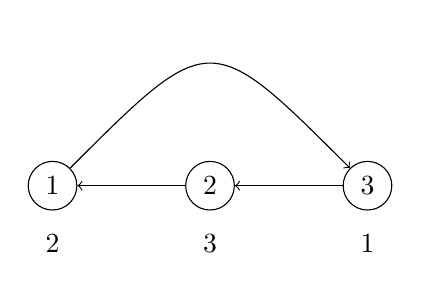
\begin{tikzpicture}[scale=1]
\path (0, 0) node[circle, draw] (1) {1}
      (2, 0) node[circle, draw] (2) {2}
      (4, 0) node[circle, draw] (3) {3};
\draw[<-] (1) edge (2)
          (2) edge (3)
          (3) .. controls (2, 2) .. (1);
\path (0, -0.5) node[below] {2}
      (2, -0.5) node[below] {3}
      (4, -0.5) node[below] {1};
\end{tikzpicture}
\caption{变换$(2\ 3\ 1)$是一个循环置换}
\label{fig:cycle-permutation}
\end{figure}

为此我们可以把置换$(2, 3, 1, 4, 5)$进一步简写为$(2\ 3\ 1)$。注意这种写法元素间没有逗号,并且认为$(1\ 2\ 3)$、$(2\ 3\ 1)$、$(3\ 1\ 2)$都表示同一个3循环置换\footnote{也有用不带空格的$(231)$来表示的,但是如果元素个数超过10个,不带空格的表示会产生歧义。可以被理解为$(23\ 1)$}。一般地,我们定义$k$-循环置换$(i_{j_1} i_{j_2} ... i_{j_k})$,它将后一个元素映射到前一个的位置,第一个元素映射到最后。组成循环:

\[
i_{j_2} \to i_{j_1}, i_{j_3} \to i_{j_2}, ..., i_{j_1} \to i_{j_k}
\]

注意,$k$-循环的元素并不一定相邻,例如$(3\ 9\ 4)$,也不一定有固定的顺序,例如$(2\ 4\ 1\ 3)$。如果循环只有两个元素$(i\ j)$称其为对调(transposition)。有个特殊情况,就是恒等置换$(1, 2, 3, 4, 5)$,我们把它记为$\epsilon = (1)$。并且有:

\[
\epsilon = (1) = (2) = ... = (n)
\]

现在我们观察置换$(2, 1, 4, 5, 3)$,它有两个循环,一个是2循环置换$(1\ 2)$,另一个是3循环置换$(3\ 4\ 5)$。为此我们可以将它表示为两个置换的乘法:

\[
(2, 1, 4, 5, 3) = (1\ 2)(3\ 4\ 5)
\]

事实上,每一个$n$元的置换$\pi$都可以写成若干个互相没有共同数字的(不相连的)循环置换的乘积。采用这种方法的好处是,虽然一般的置换是不可交换的,但是由于这样的$k$-循环置换彼此没有共同数字,所以它们是可交换的。例如$(1\ 2)(3\ 4\ 5) = (3\ 4\ 5)(1\ 2)$。

下面是$S_3$的全体循环置换用这种记法的列表:

\[
(1),
(1\ 2), (1\ 3), (2\ 3),
(1\ 2\ 3), (1\ 3\ 2)
\]

任意给一个置换$(k_1, k_2, ..., k_n)$,如何将其转化为若干个不相连的循环置换的乘积呢?我们可以按照这样的规则来操作。首先从左到右依次比较置换的每个元素,如果$k_i$和$i$相等,说明这个元素无需置换;否则先写下左括号,然后将第$k_i$个元素的值$k_j$写到括弧中,接着顺着$k_j$继续寻找,将其和$j$比较,如果不等,就写入括弧,再检查第$k_j$个元素。重复这个步骤直到发现某个元素形成了循环。这时可以写下右括号,完成一个循环。此后再继续从左向右比较置换中的元素,直到处理完所有的\cite{Armstrong1988}(27页)。如果所有的$k_i$都和$i$相等,我们可以写下$(1)$表示恒等置换。这一过程特别适合用编程的方法实现,下面就是相应的算法,和一种对应的源代码。

\begin{algorithmic}
\Function{k-cycles}{$\pi$}
  \State $r \gets []$
  \For{$i \gets 1$ to $|\pi|$}
    \State $p \gets []$
    \While{$i \neq \pi[i]$}
      \State $p \gets \pi[i]:p$
      \State Exchange $\pi[i] \leftrightarrow \pi[\pi[i]]$
    \EndWhile
    \If{$p \neq []$}
      \State $r \gets r:(\pi[i]:reverse(p))$
    \EndIf
  \EndFor
  \If{$r \neq []$}
    \State \Return r
  \Else
    \State \Return $[[1]]$ \Comment{返回恒等变换}
  \EndIf
\EndFunction
\end{algorithmic}

将任意置换转换为不相连的$k$-循环的乘积:
\lstset{language=Python}
\begin{lstlisting}
def kcycles(a):
    r = []
    n = len(a)
    for i in range(n):
        p = []
        while i + 1 != a[i]:
            p.append(a[i])
            j = a[i] - 1
            a[i], a[j] = a[j], a[i]
        if p != []:
            r.append([a[i]] + p)
    return r if r != [] else [[1]]
\end{lstlisting}

由上一小节的定理,我们有

\begin{theorem}
每一个有限群都与一个置换群同构。
\end{theorem}

这样对于任何有限群,例如方程的根,我们都可以用置换群加以研究。而置换群又是一种比较容易计算的群,这正是伽罗瓦解决方程根式解问题的方法。

\begin{Exercise}
\Question{列出$S_4$的全体元素。}
\Question{将$S_3$的所有元写成不相连的循环置换的乘积。}
\Question{编程将$k$-循环的乘积转换回置换。}
\end{Exercise}

\subsection{循环群}

\index{循环群(cyclic group)}
在各种群中,循环群(cyclic group)是最简单的。它是人们已经完全解决了的一类群。一个群$G$中的所有元素会不会都是某一个固定元素的乘方?这是有可能的。
举一个例子,我们看去掉0元素的模5乘法群。它包含4个元素\{1, 2, 3, 4\},其中2的各个乘方模5的结果如下:

\[
\begin{array}{l}
2^1 \bmod 5 = 2 \\
2^2 \bmod 5 = 4 \\
2^3 \bmod 5 = 3 \\
2^4 \bmod 5 = 1
\end{array}
\]

所以2的乘方生成了这个群中的所有元素。为此我们定义:

\begin{definition}
若一个群的每个元素都是某个固定元素$a$的乘方,称$G$为\textbf{循环群}。我们也说,$G$是由元$a$所生成的,并且用符号

\[
G = (a)
\]

来表示,$a$叫做$G$的一个生成元。
\end{definition}

我们举两个循环群的重要例子:

\begin{example}
整数加群中的全体整数都是1的“乘方”,这里的二元运算是加法,所以乘方就是不断进行相加。我们看任意正整数$m$:

\[
\begin{array}{rcll}
1^m & = & 1 \cdot 1 \cdot 1 \cdot ... \cdot 1 & \text{$m$次} \\
    & = & 1 + 1 + ... + 1 & \text{整数加群中乘法为+} \\
    & = & m &
\end{array}
\]

在整数加群中,1的逆元是-1,这是因为1 + (-1) = 0,而0是单位元。所以对任意负整数$-m$有:

\[
\begin{array}{rcll}
1^{-m} & = (-1)^m & \text{逆元} & \\
(-1)^m & = & (-1) \cdot (-1) \cdot (-1) \cdot ... \cdot (-1) & \text{$m$次} \\
       & = & -1 + (-1) + ... + (-1) & \text{整数加群中乘法为+} \\
       & = & -m &
\end{array}
\]

最后0是单位元,按照定义有$0 = 1^0$。综合上述三种情况,我们有$Z = (1)$。
\end{example}

这是一个无限循环群的例子,我们再举一个有限循环群的例子。

\begin{example}
我们看整数模$n$剩余类。我们用符号$[a]$表示整数$a$所在的剩余类。定义二元运算为模$n$的加法。

\[
[a] + [b] = [a + b]
\]

例如[3] + [4] 在模5时,结果为[2]。我们不难验证它符合结合律,单位元是[0],并且每个元素都存在逆。我们把这个群叫做整数模$n$的剩余类加群。包含元素[0], [1], ..., [$n$-1]。这个群是一个循环群,因为每个元[$i$]都可以写成$i$个[1]的乘方。

\[
[i] = [1] + [1] + ... + [1] \quad \text{$i$个}
\]
\end{example}

这两个例子不是随便选的。实际上,由这两个例子,我们已经认识了所有的循环群!因为有如下定理:

\begin{theorem}
若$G$是由元素$a$所生成的循环群,那么$G$的构造完全可以由$a$的阶来决定:
\begin{itemize}
\item 如果$a$的阶无限,那么$G$与整数加群同构;
\item 如果$a$的阶是整数$n$,那么$G$与整数模$n$剩余类加群同构。
\end{itemize}
\end{theorem}

\begin{proof}
如果$a$的阶无限,我们有$a^h = a^k$当且仅当$h = k$。否则,如果$h \neq k$,不妨令$h > k$,我们有$a^{h - k} = e$,这与$a$的阶无限矛盾。所以我们可以构造一一映射:

\[
f: a^k \to k
\]
从而建立循环群$G=(a)$到整数加群$Z$之间的同构。即:$a^ha^k \to h + k$。

如果$a$的阶是整数$n$,即$a^n = e$。这时$a^h = a^k$当且仅当$h \equiv k \mod n$的时候。我们可以构造一一映射:

\[
f: a^k \to [k]
\]

从而建立循环群$G = (a)$到整数模$n$剩余类加群间的同构。即:

\[
a^ha^k = a^{h + k} \to [h + k] = [h] + [k]
\]
\end{proof}

所以,抽象地来看,生成元的阶是无限大的循环群只有一个,生成元的阶是某个正整数的群也只有一个。至于这些循环群的构造,我们也知道得很清楚:

\begin{itemize}
\item $a$的阶无限大
  \begin{itemize}
  \item 群元素是:..., $a^{-2}, a^{-1}, a^0, a^1, a^2$, ...
  \item 群乘法是:$a^ha^k = a^{h + k}$
  \end{itemize}
\item $a$的阶是$n$
  \begin{itemize}
  \item 群元素是:$a^0, a^1, a^2, ..., a^{n-1}$
  \item 群乘法是:$a^ha^k = a^{(h + k) \bmod n}$
  \end{itemize}
\end{itemize}

\begin{Exercise}
\Question{证明循环群一定是阿贝尔群。}
\end{Exercise}

\subsection{子群}
\index{子群}

我们接下来介绍子群的概念。它可以帮助我们通过一个群的子集来推测整个群的性质。

\begin{definition}
一个群$G$的一个子集$H$叫做$G$的一个\textbf{子群},如果$H$对于$G$的乘法也构成一个群。
\end{definition}

对于任何群$G$,至少有两个子群,一个是$G$本身,另外是只包含一个单位元的集合$\{e\}$。这两个子群称为平凡子群。对于整数加群来说,偶数加群构成一个子群,而奇数和加法不构成子群(为什么?)。我们再举一个例子,考虑上一节介绍的置换群$S_3$的子集$H = \{(1), (1\ 2)\}$,$H$在置换复合乘法下构成一个子群。我们下面来验证一下:

\begin{enumerate}
\item 乘法的封闭性。$(1)(1) = (1)$, $(1)(1\ 2) = (1\ 2)$, $(1\ 2)(1) = (1\ 2)$, $(1\ 2) (1\ 2) = (1)$;其中最后一个乘法表示头两个元素对调后再对调会相当于恒等置换。
\item 结合律对$S_3$的所有元素都成立,故对$H$的元素也成立;
\item 单位元$(1) \in H$;
\item 每个元素的逆元都存在:$(1)(1) = (1)$、$(1\ 2) (1\ 2) = (1)$。
\end{enumerate}

这样依次验证群的所有性质比较麻烦,我们有一个方便的工具:

\begin{theorem}
一个群$G$的非空子集$H$构成子群的充分必要条件是:
\begin{enumerate}
\item 若任意$a, b \in H$,则$ab \in H$;
\item 任意元素$a \in H$,有$a^{-1} \in H$;
\end{enumerate}
\label{theorem:subgroup}
\end{theorem}

我们把这一定理的证明留作练习。这个定理可以直接得到一个推论,如果$H$是$G$的子群,那么$H$的单位元就是$G$的单位元,$H$中任意元素$a$的逆元就是它在$G$中的逆元。上述定理中的两个条件也可以用一个合并的条件来代替:

\begin{theorem}
一个群$G$的非空子集$H$构成子群的充分必要条件是。若任意$a, b \in H$,则$ab^{-1} \in H$。
\label{theorem:subgroup-2}
\end{theorem}

\begin{proof}
首先证明充分性,设$a, b \in H$,由上一定理的条件2,有$b^{-1} \in H$。再由条件1,有$ab^{-1} \in H$;

现在反过来证明必要性。设$a \in H$,所以$aa^{-1} = e \in H$,于是$ea^{-1} = a^{-1} \in H$;这就是前面定理中的条件1;接下来若$a, b \in H$,由刚刚证明的结果,$b^{-1} \in H$。所以$a(b^{-1})^{-1} = ab \in H$。这就证明了前面定理中的条件2。
\end{proof}

假如子集$H$是有限集,那么$H$构成子群的条件要更简单:

\begin{theorem}
一个群$G$的非空有限子集$H$构成子群的充分必要条件是。若任意$a, b \in H$,则$ab \in H$。
\end{theorem}

我们曾经利用一个整数$n$把全体整数分成模$n$的剩余类。我们可以把类似的思路扩展抽象到群上。我们把整数加群叫做$Z$,把所有包含$n$的倍数的集合叫做$H$,即$H = {kn}$,其中$k = 0, \pm 1, \pm 2, ...$。那么对于$H$的任意两个元$hn$和$kn$来说,$hn + (-k)n = (h - k)n \in H$。而$-kn$恰好是$kn$在$Z$中的逆元,并且$+$是整数加群上的二元运算。所以由上述定理\ref{theorem:subgroup-2},$H$是$Z$的子群。

当我们把整数划分成模$n$剩余类时,所利用的等价关系是这样规定的:

\[
a \equiv b \mod n, \text{当且仅当} n | (a - b)
\]

利用子群$H$,这一等价关系也可以这样定义:

\[
a \equiv b \mod n, \text{当且仅当} (a - b) \in H
\]

这样,我们就利用子群$H$实现了$Z$的剩余类划分。我们现在将这一情形推广到利用子群$H$对一个群$G$进行分类。为此,我们需要先用子群定义元素的一种等价关系$\sim$:

\[
a \sim b, \text{当且仅当} ab^{-1} \in H
\]

给了$a$和$b$,我们可以唯一确定$ab^{-1}$是不是属于$H$。为什么说$\sim$是一种等价关系呢?因为它满足等价关系的全部三条性质:

\begin{enumerate}
\item 因为$aa^{-1} = e \in H$,所以$a \sim a$。也就是自反性成立;
\item 如果$ab^{-1} \in H$,则它的逆$(ab^{-1})^{-1}= ba^{-1} \in H$,所以$a \sim b \Rightarrow b \sim a$。也就是对称性成立;
\item 若$ab^{-1} \in H, bc^{-1} \in H$,我们有$(ab^{-1})(bc^{-1}) = ac^{-1} \in H$,所以$a \sim b, b \sim c \Rightarrow a \sim c$。也就是传递性成立。
\end{enumerate}

\index{右陪集(right coset}
\begin{definition}
由这一等价关系$\sim$所决定的类叫做子群$H$的\textbf{右陪集}(right coset),包含元素$a$的右陪集用符号$Ha$来表示。
\end{definition}

具体来说,用$a$从右边去乘$H$的每个元素,就得到了包含$a$的类。所以$Ha$正好包含所有可以写成$ha$,其中$h \in H$形式的$G$中的元素,即:

\[
Ha = \{ha | h \in H\}
\]

\begin{figure}[htbp]
\centering
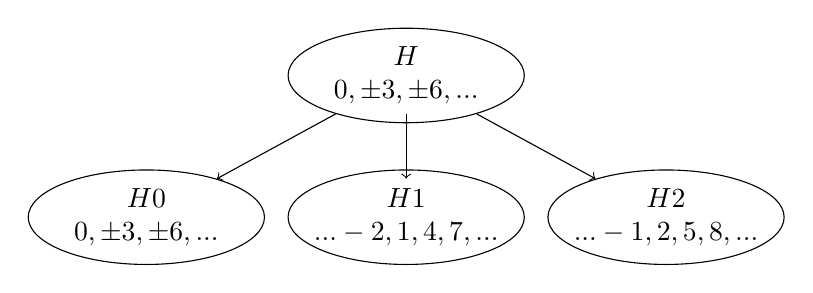
\begin{tikzpicture}[scale=0.6]
\draw (0, 3) circle[x radius=2.5cm, y radius=1cm] node[align=center] (H) {$H$ \\ $0, \pm 3, \pm 6, ...$}
      (-5.5, 0) circle[x radius=2.5cm, y radius=1cm] node[align=center] (H0) {$H0$ \\ $0, \pm 3, \pm 6, ...$}
      (0, 0) circle[x radius=2.5cm, y radius=1cm] node[align=center] (H1) {$H1$ \\ $... -2, 1, 4, 7, ...$}
      (5.5, 0) circle[x radius=2.5cm, y radius=1cm] node[align=center] (H2) {$H2$ \\ $... -1, 2, 5, 8, ...$};
\draw[->] (H) edge (H0)
          (H) edge (H1)
          (H) edge (H2);
\end{tikzpicture}
\caption{右陪集。整数加群的子群$H$包含所有3的倍数,用0、1、2分别加所有3的倍数可以得到三个互不相交子集。它们恰好是整数的一个分类。}
\label{fig:right-cosets-Z3}
\end{figure}

如图\ref{fig:right-cosets-Z3}所示,令$Z$为整数加群,$H$为所有3的倍数$0, \pm 3, \pm 6, ...$,它在加法下构成一个子群。我们用$Z$中的元素0从右侧加\footnote{由于整数加群是阿贝尔群,加法满足交换律,所以左右陪集相同。}$H$中的每个元素得到$H0$,显然这一结果还等于$H$,是所有模3余0的整数,记为[0];用$Z$中的元素1从右侧加$H$中的每个元素得到$H1$,它包含所有模3余1的整数,记为[1];用$Z$中的元素2从右侧加$H$中的每个元素得到$H2$,它包含所有模3余2的整数,记为[2]。如果用3加所有$H$的元素,结果和$H0$一样。事实上,如果我们用$H0$中的任何元素$a$获得的右陪集$Ha$都等于$H0$;用$H1$中的任何元素$b$获得的右陪集$Hb$都等于$H1$,用$H2$中的任何元素$c$获得的右陪集$Hc$都等于$H2$。$H0$、$H1$、$H2$三个右陪集放在一起恰好是全体整数$Z$。它们的确是$Z$的一个分类:[0], [1], [2]。

\begin{figure}[htbp]
\centering
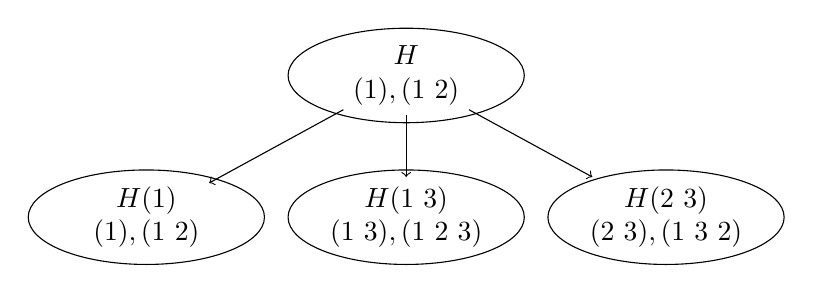
\begin{tikzpicture}[scale=0.6]
\draw (0, 3) circle[x radius=2.5cm, y radius=1cm] node[align=center] (H) {$H$ \\ $(1), (1\ 2)$}
      (-5.5, 0) circle[x radius=2.5cm, y radius=1cm] node[align=center] (H1) {$H(1)$ \\ $(1), (1\ 2)$}
      (0, 0) circle[x radius=2.5cm, y radius=1cm] node[align=center] (H13) {$H(1\ 3)$ \\ $(1\ 3), (1\ 2\ 3)$}
      (5.5, 0) circle[x radius=2.5cm, y radius=1cm] node[align=center] (H23) {$H(2\ 3)$ \\ $(2\ 3), (1\ 3\ 2)$};
\draw[->] (H) edge (H1)
          (H) edge (H13)
          (H) edge (H23);
\end{tikzpicture}
\caption{有限非阿贝尔群的右陪集。}
\label{fig:right-cosets-S3}
\end{figure}

我们再看一个有限非阿贝尔群的例子。考虑3阶置换群

$G = S_3 = \{(1), (1\ 2), (1\ 3), (2\ 3), (1\ 2\ 3), (1\ 3\ 2)\}$,

及其子群$H = \{(1), (1\ 2)\}$。我们用单位元恒等置换$(1)$,和另外两个置换$(1\ 3)$、$(2\ 3)$右乘$H$得到3个右陪集:

\[
\begin{array}{rcl}
H(1) & = & \{(1), (1\ 2)\} \\
H(1\ 3) & = & \{(1\ 3), (1\ 2\ 3)\} \\
H(2\ 3) & = & \{(2\ 3), (1\ 3\ 2)\}
\end{array}
\]

我们也可以用另外三个元来作右陪集:

$H(1\ 2)$、$H(1\ 2\ 3)$、$H(1\ 3\ 2)$

同样由于
$(1\ 2) \in H(1)$、$(1\ 2\ 3) \in H(1\ 3)$、$(1\ 3\ 2) \in H(2\ 3)$,所以一定有

\[
\begin{array}{l}
H(1) = H(1\ 2) \\
H(1\ 3) = H(1\ 2\ 3) \\
H(2\ 3) = H(1\ 3\ 2)
\end{array}
\]

这样,子群$H$把整个群$G = S_3$分成$H(1)$、$H(1\ 3)$、$H(2\ 3)$三个不同的右陪集,这三个右陪集放在一起正是$G$,它们是$G$的一个分类。

\index{左陪集}
与右陪集对称,我们也可以定义左陪集。规定对称的等价关系$\sim'$:

\[
a \sim' b \text{当且仅当} b^{-1}a \in H
\]

这样,由等价关系$\sim'$所决定的类叫做子群$H$的左陪集。包含元素$a$的左陪集用符号$aH$来表示。它包含所有形如:$ah, h \in H$形式的$G$的元。因为一个群的乘法不一定满足交换律,所以一般来说$\sim$和$\sim'$两个等价关系并不相同,$H$的左右陪集也不相同。但是一个子群的左右陪集之间有一个共同点:

\begin{theorem}
子群$H$的左右陪集个数相等,他们或者都是无限大,或者都有限并相等。
\end{theorem}

要想证明这一点,我们可以构造一个从$H$的右陪集到左陪集间的映射:$f: Ha \to a^{-1}H$。容易验证,这是一个一一映射。任意$Ha = Hb$,都有$ab^{-1} \in H$,所以$(ab^{-1})^{-1} = ba^{-1} \in H$。因此$a^{-1}H= b^{-1}H$。既然一一映射存在,自然左右陪集的个数是相等的。

为此,我们可以将子群$H$的陪集个数(左或者右)定义为$H$在$G$中的\textbf{指数}。

一般情况下,子群的右陪集$Ha$未必等于左陪集$aH$,如果相等,这是的子群叫做正规子群。正是伽罗瓦第一个引入了正规子群来分析方程的可解性。

\index{正规子群} \index{不变子群}
\begin{definition}
一个群$G$的子群$N$叫做一个\textbf{正规子群}(或者不变子群),加入对$G$的每个元$a$都有:
\[
Na = aN
\]
一个正规子群的左(或右)陪集叫做$N$的\textbf{陪集}。
\label{normal-subgroup}
\end{definition}

由于其对称性,正规子集也叫做群的中心。判断一个群是否是正规子群,我们有以下两个定理:

\begin{theorem}
一个群$G$的子群$N$是一个不变子群的充分必要条件是对$G$中的任何一个元$a$都有:
\[
aNa^{-1} = N
\]
\end{theorem}

\begin{theorem}
一个群$G$的子群$N$是一个不变子群的充分必要条件是对$G$中的任何一个元$a$,$N$中的任何一个元$n$都有:
\[
ana^{-1} \in N
\]
\end{theorem}

我们可以把正规子群$N$的所有陪集做成一个集合$\{aN, bN, cN, ...\}$,并且定义这个集合上的乘法为:

\[
(xN)(yN) = (xy)N
\]

\index{商群}
可以验证,正规子群的陪集在这个乘法下构成一个群,叫做\textbf{商群},用$G/N$表示。在正规子群、商群和同态映射之间存在着重要的关系。首先一个群$G$同它的每个商群$G/N$同态。要证明这一点,我们可以构造一个映射$a \to aN, a \in G$。这显然是一个从$G$到商群的满射,对于$G$中任何两个元素$a, b$,都有$ab \to abN = (aN)(bN)$。所以它是一个同态满射。这样我们既可以通过正规子群,也可以通过商群推测群$G$的性质。为了做到这一点,我们定义一下“核”的概念。

\index{核}
\begin{definition}
若$f$是群$G$到另一个群$G'$的同态满射,$G'$的单位元$e'$在映射$f$之下的逆像集合是$G$中的一个子集。这个子集叫做同态满射$f$的\textbf{核}。
\end{definition}

我们有如下定理,如果$G$和$G'$同态,那么这个同态满射的核$N$是$G$的正规子群。并且其商群$G/N \cong G'$。这样一个群不仅和和它的每一个商群同态,并且抽象地来看,$G$只能和它的商群同态。有时候,我们发现群$G$和$G'$同态,但是$G'$的性质我们并不清楚,这时候,我们一定能找到$G$的一个正规子群$N$,使得$G'$的性质和商群$G/N$完全一样。从这里我们能看出不变子群和商群的意义。伽罗瓦正是通过这一点,想出并定义了方程的群的可解性。

\begin{Exercise}
\Question{证明子群的判定定理\ref{theorem:subgroup}。}
\Question{列出图\ref{fig:right-cosets-S3}中$H$的左陪集。}
\end{Exercise}

\subsection{拉格朗日定理}
\index{拉格朗日}

拉格朗日定理是特别体现抽象代数特点的一个定理。在完全无须了解群中元素和运算的具体意义的情况下,我们仍可以揭示抽象结构的内在规律。

%\begin{figure}[htbp]
\begin{wrapfigure}{R}{0.4\textwidth}
 \raggedright %\centering
 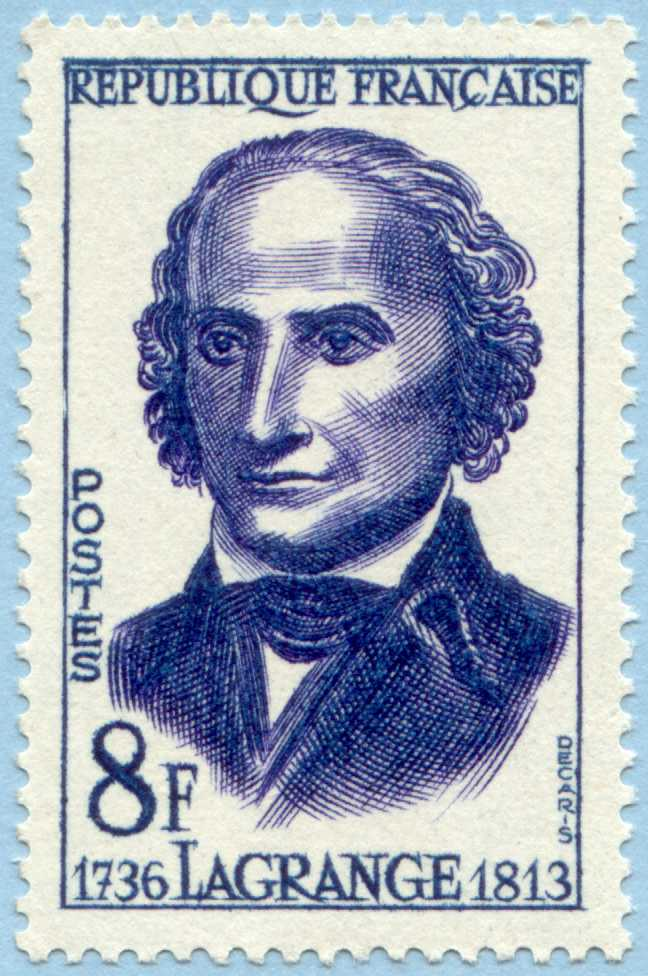
\includegraphics[scale=1.5]{img/lagrange.eps}
 \captionsetup{labelformat=empty}
 \caption{拉格朗日纪念邮票}
 \label{fig:Lagrange}
\end{wrapfigure}
%\end{figure}

% 拉格朗日(Joseph-Louise Lagrange)
拉格朗日全名为约瑟夫$\cdot$路易斯$\cdot$拉格朗日,是法国著名数学家、物理学家。1736年1月25日生于意大利都灵。拉格朗日的祖先是法国军官,到意大利后与罗马家族的人结婚定居。他的父亲曾任都灵的公共事务和防务局会计,但后来由于经商破产,家道中落。据拉格朗日本人回忆,如果幼年时家境富裕,他也就不会作数学研究了,因为父亲一心想把他培养成为一名律师。拉格朗日在都灵大学读书时,并没有对数学发生兴趣,他觉得欧几里得几何很枯燥。

17岁时,拉格朗日碰巧看到了英国天文学家哈雷的一篇介绍牛顿微积分的文章。他一下子被吸引住了。开始全身心投入学习数学。1755年拉格朗日19岁时,在探讨数学难题“等周问题”的过程中,他以欧拉的思路和结果为依据,用纯分析的方法求变分极值。第一篇论文“极大和极小的方法研究”,发展了欧拉所开创的变分法,为变分法奠定了理论基础。变分法的创立,使拉格朗日在都灵声名大振,并使他在19岁时就当上了都灵皇家炮兵学校的教授,成为当时欧洲公认的第一流数学家。1756年,受欧拉的举荐,拉格朗日被任命为普鲁士科学院通讯院士。

1766年德国的腓特烈大帝向拉格朗日发出邀请时说,在“欧洲最大的王”的宫廷中应有“欧洲最大的数学家”。于是他应邀前往柏林,任普鲁士科学院数学部主任,居住达20年之久,开始了他一生科学研究的鼎盛时期。在此期间,他完成了《分析力学》一书,这是牛顿之后的一部重要的经典力学著作。书中运用变分原理和分析的方法,建立起完整和谐的力学体系,使力学分析化了。

腓特烈大帝非常欣赏拉格朗日,常常和他谈论规律生活的重要性。在皇帝的影响下,拉格朗日每天晚上都想好明天要完成的具体任务。每当工作取得进展,他都写一段简短的分析看看哪里还能进一步改进。拉格朗日在撰写论文前总是深思熟虑,他通常能一气呵成而不用修改。但拉格朗日不太习惯柏林的气候,他的身体一直不太好。1783年,他的妻子维多利亚因病去世。

1786年一直支持他的腓特烈大帝也去世了。拉格朗日接受了路易十六的邀请来到巴黎。他得到了特别的接待,国王甚至在卢浮宫里为他安排了一处住所。1792年,拉格朗日的朋友,天文学家勒莫尼埃(LeMonnier)的女儿,24岁蕾妮(Renée-Francoise- Adelaide)坚持要嫁给孤单一人的拉格朗日。他们结婚后虽未生儿女,但家庭幸福。

这时法国大革命爆发了。1793年9月革命政府决定逮捕所有在敌国出生的人,著名化学家拉瓦锡在身处危险的情况下竭力奔走相助,终于才把拉格朗日作为例外。1794年5月4日法国雅各宾派开庭审判波旁王朝税务人员,把包括拉瓦锡在内的28名成员全部处以死刑。拉格朗日等人尽力地挽救,请求赦免,但是遭到了革命法庭副长官考费那尔(J.B.Coffinhal)的拒绝,全部予以驳回,并宣称,“共和国不需要学者,而只需要为国家而采取的正义行动!”5月8日早晨,拉格朗日痛心地说:“他们可以一眨眼就把拉瓦锡的头砍下来,但他那样的头脑一百年也再长不出一个来了。”\cite{Wiki-Lagrange}

1799年雾月政变后,拿破仑热情支持法国的科学研究。他提名拉格朗日等著名科学家成为上议院议员及新设的勋级会荣誉军团成员,封为伯爵;还在1813年4月3日授予他帝国大十字勋章。此时拉格朗日已重病在身,终于在4月11日晨逝世。在葬礼上,由议长拉普拉斯代表上议院,院长拉赛佩德(Lacépède)代表法兰西研究院致悼词。意大利各大学都举行了纪念活动。

拉格朗日是18世纪的伟大科学家,在数学、力学和天文学三个学科中都有历史性的重大贡献。但他主要是数学家,拿破仑曾称赞他是“一座高耸在数学界的金字塔”,他最突出的贡献是在把数学分析的基础脱离几何与力学方面起了决定性的作用。使数学的独立性更为清楚,而不仅是其他学科的工具。同时在使天文学力学化、力学分析化上也起了历史性作用,促使力学和天文学(天体力学)更深入发展。

拉格朗日在柏林的前十年,把大量时间花在代数方程和超越方程的解法上。他在代数方程解法中有历史性贡献。他把前人解三、四次代数方程的各种解法,总结为一套标准方法,而且还分析出一般三、四次方程能用代数方法解出的原因。三次方程有一个二次辅助方程,其解为三次方程根的函数,在根的置换下只有两个值;四次方程的辅助方程的解则在根的置换下只有三个不同值,因而辅助方程为三次方程。拉格朗日称辅助方程的解为原方程根的预解函数(是有理函数)。他继续寻找5次方程的预解函数,希望这个函数是低于5次的方程的解,但没有成功。尽管如此,拉格朗日的想法已蕴含着置换群概念,而且使预解(有理)函数值不变的置换构成子群,子群的阶是原置换群阶的因子。这正是群论中著名的拉格朗日定理。拉格朗日是群论的先驱。他的思想为后来的阿贝尔和伽罗瓦采用并发展,终于解决了五次以上的一般方程为何不能用代数方法求解的问题。

在介绍拉格朗日定理前,我们首先看一个引理:

\begin{lemma}
一个子群$H$与其每一个右陪集$Ha$之间都存在一一映射。
\end{lemma}

由于陪集的左右对称性,这一结论对于左陪集也成立。要想证明它,我们可以构造映射$f: h \to ha$,它就是一个从子群到右陪集的一一映射,因为:

\begin{enumerate}
\item $H$中的每个元素$h$都有一个唯一的像$ha$;
\item $Ha$中的每个元素$ha$都是子群$H$中元素$h$的像;
\item 任意$h_1a = h_2a$,都有$h_1 = h_2$。
\end{enumerate}

由于一一映射的存在,我们知道有限群$G$中,陪集中元素的个数一定与子群$H$的阶相等。而且由于陪集的分类特性,我们知道群中的每个元素都可以在某一个陪集中找到。这样我们就可以利用陪集发现子群$H$与有限群$G$之间的一个关系:

\index{拉格朗日定理}
\begin{theorem}
\textbf{拉格朗日定理}:有限群$G$的阶,能够被其子群$H$的阶整除。
\end{theorem}

\begin{proof}
首先,我们知道$G$能够为$H$的陪集全部覆盖;并且由于陪集之上定义的等价关系,我们知道陪集之间是没有交集的。如果存在元素$c$既属于$Ha$,也属于$Hb$,那么$c \sim a$,$c \sim b$,所以$a \sim b$,所以$Ha = Hb$。再加上子群$H$与陪集存在一一映射的引理,我们知道每个陪集的大小都等于$H$的阶$|H|=n$,如果陪集的个数(也就是$H$的指数)等于$m$,一定有
\[
|G| = mn
\]
\end{proof}

注意,拉格朗日定理的逆定理不一定成立。我们无法将群的阶做任意因子分解,然后对每个因子都找到子群和陪集。从拉格朗日定理,我们可以得到很多有用的推论。

\begin{corollary}
一个有限群$G$中的任意元素$a$的阶都能整除$G$的阶。
\end{corollary}

这是因为$a$生成一个阶为$n$的子群,所以$n$能整除$|G|$。

\begin{corollary}
如果$G$的阶是素数,那么$G$是循环群。
\end{corollary}

这是因为任何不等于单位元的元素$a$,它所生成的子群的阶一定等于$G$的阶。所以$a$是$G$的生成元,即$G = (a)$。

\begin{corollary}
有限群$G$中的任何元素$a$,都有$a^{|G|} = e$。
\label{corollary:Lagrange-elem-order}
\end{corollary}

这是因为$a$的阶$n$能够整除$G$,不妨令$|G| = nk$。所以
\[
a^{|G|} = a^{nk} = (a^n)^k = e^k = e
\]

群论中的拉格朗日定理可以用来证明数论中著名的费马小定理和欧拉定理。费马小定理是法国数学家费马于1636年发现的。他在1640年10月18日写给友人\footnote{费马的朋友法国数学家贝西(Bernard Frénicle de Bessy)}的信中首次提出了这个定理。1736年,欧拉给出了费马小定理的一个证明。但从莱布尼茨未发表的手稿中发现他在1683年以前已经得到几乎相同的证明。

\index{费马小定理}
\begin{theorem}
\textbf{费马小定理}:若$p$是素数,对任何满足$0 < a < p$的整数$a$都有,$a^{p-1}-1$能被$p$整除。
\end{theorem}

\begin{proof}
考虑整数模$p$乘法群。这个群的元素由所有模$p$的非零余数构成,因为$p$是素数,所以群元素为1, 2, ..., $p-1$,单位元$e = 1$,群的阶为$p-1$。根据拉格朗日定理的推论\ref{corollary:Lagrange-elem-order},有:
\[
a^{p-1} = e
\]
因为单位元为1,所以上式可写为:
\[
a^{p-1} \equiv 1 \mod p
\]
故$p$整除$a^{p-1} - 1$。
\end{proof}

和这一证明对比,初等数论方法的证明要复杂得多(\cite{StepanovRose15}第5.2到5.4)。我们再介绍另一种有趣的“项链”证法\cite{Wiki-FLT-proof},供读着参考。

\begin{proof}
考虑有$a$颗不同颜色的珍珠,我们要串一条长为$p$的珍珠串。其中$p$为素数。显然一共有$a^p$种不同的串,这是因为串中每个位置都可以在$a$颗珍珠中选择,共选$p$次。

例如有两种颜色$A$、$B$的珍珠,要串长度为5的串。即$a = 2, p = 5$,一共有$2^5 = 32$种不同的串:

\begin{verbatim}
  AAAAA, AAAAB, AAABA, ..., BBBBA, BBBBB.
\end{verbatim}

我们要证明,在这$a^p$串珍珠中,如果去掉$a$个颜色完全相同的串(在上述例子中是串\texttt{AAAAA}和\texttt{BBBBB}),剩下的$a^p - a$串珍珠可以分成若干组,每个组恰好有$p$串珍珠。也就是说$p$整除$a^p - a$。

如果把每串珍珠首尾连接起来做成项链。原来有些不同的串会变成相同的项链。如果一个串可以通过旋转变换成另一个,这两个串必然做成相同的项链。例如下面的5个串珍珠可以做成相同的项链:

\begin{verbatim}
  AAAAB, AAABA, AABAA, ABAAA, BAAAA.
\end{verbatim}

\begin{figure}[htbp]
  \centering
  \subcaptionbox{一串项链代表7种不同的串:\texttt{ABCBAAC}, \texttt{BCBAACA}, \texttt{CBAACAB}, \texttt{BAACABC}, \texttt{AACABCB}, \texttt{ACABCBA}, \texttt{CABCBAA}}[0.45\linewidth]{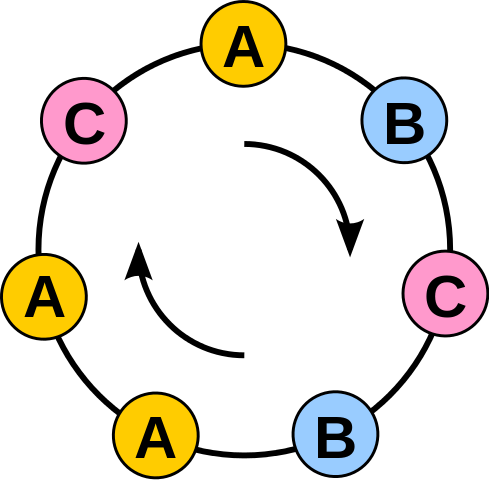
\includegraphics[scale=0.2]{img/bracelet-rotate.eps}} \quad
  \subcaptionbox{相同珍珠串成的项链只代表一种串:\texttt{AAAAAAA}}[0.45\linewidth]{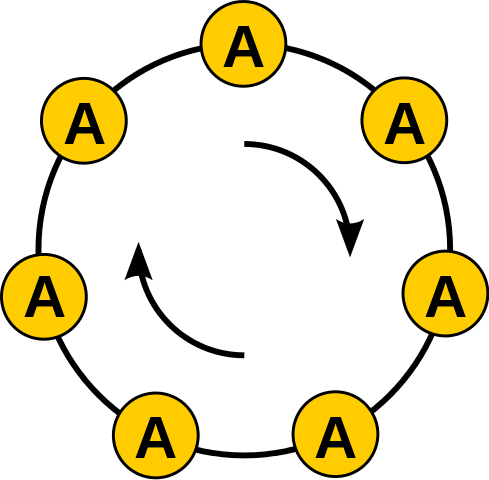
\includegraphics[scale=0.2]{img/bracelet-identical.eps}}
  \caption{通过项链对珍珠串进行分类}
  \label{fig:bracelet}
\end{figure}

用这种方法,上面例子中的32串珍珠可以分成5种不同颜色的项链和2种同色的项链:

\begin{verbatim}
  [AAABB, AABBA, ABBAA, BBAAA, BAAAB];
  [AABAB, ABABA, BABAA, ABAAB, BAABA];
  [AABBB, ABBBA, BBBAA, BBAAB, BAABB];
  [ABABB, BABBA, ABBAB, BBABA, BABAB];
  [ABBBB, BBBBA, BBBAB, BBABB, BABBB];
  [AAAAA];
  [BBBBB].
\end{verbatim}

一串项链可以代表多少种不同的串呢?如果一个串$S$由若干相同的子串$T$复制连接而成,而$T$无法再继续分拆成相同的子串,则由$S$构成的项链可代表$|T|$种不同的串,其中$|T|$表示串$T$的长度。例如串$S=$\texttt{ABBABBABBABB},由相同的子串$T=$\texttt{ABB}复制多次而成,如果我们一次旋转一颗珍珠,一共可以得到3串不同的结果:

\begin{verbatim}
  ABBABBABBABB,
  BBABBABBABBA,
  BABBABBABBAB.
\end{verbatim}

除去这3种之外,不可能再有其它不同种类的串了。\texttt{ABB}的长度为3,再次旋转必然会循环得到相同的结果。这样,所有的$a^p$串珍珠可分成两类。一类是$a$串颜色相同的串;另一类颜色不同,但是由于这些串的长度$p$是素数,它绝不可能由若干子串复制连接出来。所以任何一个这样的串连成的项链,总共代表$p$种不同的串。而这样的串总共有$a^p - a$种,它们可以通过连成项链后分组,每组恰好$p$个串,代表一种不同的项链。因此$a^p-a = a^{p-1}$一定可以被$p$整除。
\end{proof}

项链证明法可能是费马小定理已知证法中最容易的,它不需要太多的数学知识。核心思想是利用两种不同的方式数数的结果必然是一样的。

%\begin{figure}[htbp]
\begin{wrapfigure}{L}{0.35\textwidth}
  \centering %\raggedleft
 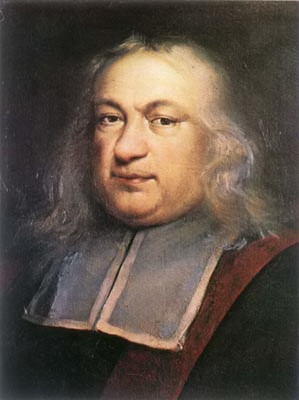
\includegraphics[scale=0.4]{img/Fermat.eps}
 \captionsetup{labelformat=empty}
 \caption{皮埃尔$\cdot$德$\cdot$费马 1601-1665}
 \label{fig:Fermat}
\end{wrapfigure}
%\end{figure}

费马小定理从提出到欧拉成功证明经过了整整100年。这是费马的一贯风格,费马大定理(也称费马的最后定理)难住了无数天才数学家,历经358年才由英国数学家安德鲁$\cdot$怀尔斯在1995年成功攻克。而怀尔斯的主要武器包括椭圆曲线、模形式和伽罗瓦表示\cite{HanXueTao2009}。可以说费马留下的这些猜想是一笔丰富的数学遗产。

\vspace{5mm}

\index{费马(Pierre de Fermat )}
费马是法国著名数学家,1601年8月生于法国图卢兹一个富有的皮革商人家中。他是一位全职律师,一直在司法部门工作,后来还当过图卢兹最高法院的大法官。费马在成年后才开始利用业余时间研究数学。但费马取得的数学成就,堪称那个时代的高峰。1630年,费马独立得到了解析几何的基本原理\footnote{费马的8页论文《平面与立体轨迹引论》在1630年完成,但在1679年费马死后14年才出版。},因而与笛卡尔分享创立解析几何的荣誉;他与帕斯卡在一段漫长而有趣的通信中一起奠定了古典概率论的基础,提出了数学期望的概念,因而与帕斯卡被公认为是概率论的创始人;他提出光学中的“费马原理”\footnote{又称最小作用原理,或最短时间作用原理。},给后来变分法的研究以极大的启示;他是创建微积分学的杰出先驱者。而费马本人最感兴趣的领域是数论。

费马对数论的兴趣是由古希腊数学家丢番图的名著《算术》启发的。1621年,巴谢(Bachet)校订注释的希腊——拉丁文对照本在法国出版。费马在巴黎买到此书,并被其中的数论问题深深吸引。值得庆幸的是,这一版的每一页都留有宽大的空白页边,于是这书同时成了费马的笔记本。在研究丢番图的问题和解答时,他会受到启发去思考和解决更多、更深入的问题,并草草地在这些空白书边上写下自己的评注。

费马在其生前,几乎没有公开发表过任何他的数学成果。这在“不发表就发霉”的今天是很难被理解的。除了把自己的研究成果写在书籍的页边,费马也常常按照当时流行的风气,以书信的形式向一些学者朋友报告。究其原因,费马是被“发现新的数学奥秘”这类强烈的念头所驱使的。研究数学对于他是一种消遣,纯粹是由于他对数学的爱好。当创造出他从未触及的结果时,费马会获得真正的愉悦与自我满足。因而公开发表和被人们承认对他而言没有多大意义\cite{HanXueTao2009}。有趣的是,这位缄默的天才有时喜好捉弄人,他经常在信中向其他数学家发出挑战,要求他们证明自己发现的某些数学结果。

\begin{wrapfigure}{R}{0.33\textwidth}
%\begin{figure}[htbp]
 \centering
 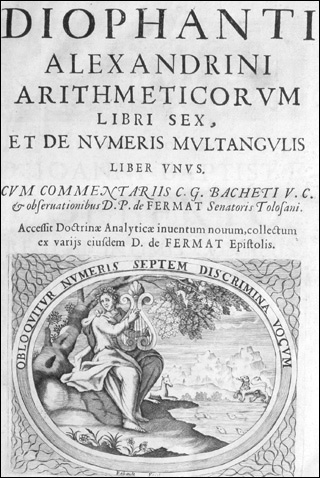
\includegraphics[scale=0.5]{img/Arithmetica.eps}
 \captionsetup{labelformat=empty}
 \caption{丢番图《算术》1670年版,带有费马评注}
 \label{fig:Arithmetica}
%\end{figure}
\end{wrapfigure}

当费马在1665年1月去世时,他的研究成果散落各处。费马的长子塞缪尔(Samuel)花了5年时间整理信件收集注记,1670年将他父亲的成果出版为一个特殊版本的《算术》。在封面图片上方,写着“附有费马的评注”的小字。这一版本包括费马所做的48个评注。1679年,他又整理了出版了费马的第二卷著作。费马生前的这些研究成果终于得以流传,极大地丰富了十七世纪的数学宝库,推动了后来的数学发展。

在费马之前,数论基本上是一些相关问题的汇集。费马振兴了数论的研究,系统地提出了数量众多的数论定理,并引入了一般化的方法和原理,从而把数论引上了近代发展的轨道。可以说,正是费马的系统化工作,数论才真正开始成为一门数学分支。费马也因此奠定近代数论的基础,而被称为“近代数论之父”。在高斯的《算术研究》出版之前,数论的发展始终是跟费马的推动联系在一起的。

然而,费马生前提出的种种结论常常仅含有证明的一些关键部分,有时甚至根本没有证明。有些内容后来发现是错误的\footnote{例如费马数。费马在1640年宣称$2^{2^n}+1$形式的数都是素数,并且当$n$为0, 1, 2, 3, 4时都是对的。它们分别是3, 5, 17, 257, 65537。但欧拉在1732年算出$2^{2^5} + 1 = 641 \times 6700417$。目前(2017年)人们已经找到243个反例,却没有再发现第6个费马素数。是否还有其它费马素数至今没有人能够解决。}。因此在找到严格的数学证明前,这些结论只能称之为“猜想”。这些猜想有很多是被欧拉攻克的,不仅如此,欧拉还在费马的基础上发展了更多的结果。

我们接下来要介绍的数论中的欧拉定理,就是比费马小定理更加普遍的结果。在成功证明了费马小定理后,欧拉并不满足,如果$p$不是素数会怎样呢?欧拉仔细研究了合数的情况,得出并证明了下面的定理。

\index{欧拉定理} \index{欧拉函数}
\begin{theorem}
\textbf{欧拉定理}:如果$0 < a < n$且$a$与$n$互素,那么$a^{\upphi(n)} - 1$能够被$n$整除。
\end{theorem}

其中$\upphi(n)$是欧拉函数\footnote{也称为欧拉总计函数(Euler totient function)或者欧拉$\upphi$函数},它的定义是所有小于$n$且与$n$互素的正整数个数。即:

\[
\upphi(n) = |\{i | 0 < i < n\ \text{且} gcd(i, n) = 1 \}|
\]

欧拉使用初等数论的方法证明了这一定理。我们展示如何利用群论和拉格朗日定理给出一个简洁的证明。

\begin{proof}
考虑整数模$n$的非零余数。我们把模$n$乘法之下可以互逆的所有余数挑选出来。它们构成一个模$n$乘法群。按照欧拉$\upphi$函数的定义,$\upphi(n)$的值,是所有小于$n$且与$n$互素的正整数的个数。而这些正整数,恰好对应这个乘法群中的元素。所以这个群的阶就是$\upphi(n)$。根据拉格朗日定理的推论\ref{corollary:Lagrange-elem-order},有:

\[
a^{\upphi(n)} = e
\]

故而$a^{\upphi(n)} \equiv 1 \mod n$,所以$n$一定整除$a^{\upphi(n)} - 1$。
\end{proof}

我们举个例子,下表是模10的非零余数的乘法表。我们可以从表中找到单位元1,用下划线标出。然后从其所对应的行列找到模乘的两个数,加粗标出。这些数都和10互素。反之,那些不和10互素的余数所在的行列中都有0元素,而0不是群中的元。可以看到和10互素的余数恰好是群中的元素1, 3, 7, 9。

\vspace{5mm}
\definecolor{Gray}{gray}{0.9}
\newcolumntype{g}{>{\columncolor{Gray}}c}
\begin{tabular}{c|g|c|g|c|c|c|g|c|g|}
  & \textbf{1} & 2 & \textbf{3} & 4 & 5 & 6 & \textbf{7} & 8 & \textbf{9} \\
\hline
\rowcolor{Gray}
\textbf{1} & \cellcolor{gray} \underline{1} & 2 & 3 & 4 & 5 & 6 & 7 & 8 & 8 \\
\hline
2 & 2 & 4 & 6 & 8 & 0 & 2 & 4 & 6 & 8 \\
\hline
\rowcolor{Gray}
\textbf{3} & 3 & 6 & 9 & 2 & 5 & 8 & \cellcolor{gray}\underline{1} & 4 & 7 \\
\hline
4 & 4 & 8 & 2 & 6 & 0 & 4 & 8 & 2 & 6 \\
\hline
5 & 5 & 0 & 5 & 0 & 5 & 0 & 5 & 0 & 5 \\
\hline
6 & 6 & 2 & 8 & 4 & 0 & 6 & 2 & 8 & 4 \\
\hline
\rowcolor{Gray}
\textbf{7} & 7 & 4 & \cellcolor{gray} \underline{1} & 8 & 5 & 2 & 9 & 6 & 3 \\
\hline
8 & 8 & 6 & 4 & 2 & 0 & 8 & 6 & 4 & 2 \\
\hline
\rowcolor{Gray}
\textbf{9} & 9 & 8 & 7 & 6 & 5 & 4 & 3 & 2 & \cellcolor{gray} \underline{1} \\
\hline
\end{tabular}
\vspace{5mm}

任给一个整数$n$,如何求出其欧拉函数的值呢?因为任何大于1的整数都可以写成素数幂的乘积形式,我们首先来看,对于素数$p$的$m$次幂,$\upphi(p^m)$如何计算。也就是求出从1到$p^m-1$中,有多少个数和$p^m$互素。显然我们只要把$p$的倍数这些数除去即可。这些数分别是:$p, 2p, 3p, ..., p^m - p$,我们把它们分别除以$p$,就可以得到自然数序列:$1, 2, 3, ..., p^{m-1} - 1$。显然共有$p^{m-1} - 1$个。于是素数的整数次幂的欧拉函数值为:

\[
\begin{array}{rcl}
\upphi(p^m) & = & (p^m - 1) - (p^{m-1} - 1) \\
            & = & p^m - p^{m-1} \\
            & = & p^m(1-\dfrac{1}{p})
\end{array}
\]

接下来我们考虑$n = p^uq^v$,也就是两个不同素数幂的积。我们首先从1到$n-1$中,减去$p$的所有倍数,然后再减去$q$的所有倍数,但是有些整数既是$p$的倍数,也是$q$的倍数,所以最后要把这些$pq$的倍数再加回来(组合中的容斥原理)。这样有:

\[
\begin{array}{rcl}
\upphi(p^uq^v) & = & (n - 1) - (\dfrac{n}{p} - 1) - (\dfrac{n}{q} - 1) + (\dfrac{n}{pq} - 1) \\
          & = & n(1 - \dfrac{1}{p})(1 - \dfrac{1}{q}) \\
          & = & p^u(1 - \dfrac{1}{p})q^v(1 - \dfrac{1}{q}) \\
          & = & \upphi(p^u)\upphi(p^v)
\end{array}
\]

特别地,当指数$u$, $v$都是1的时候,我们有$\upphi(pq) = \upphi(p)\upphi(q)$。并且我们可以把这个结果推广到多个素数幂的情况,如果$n = p_1^{k_1}, p_2^{k_2}...p_m^{k_m}$,则其欧拉函数的值为:

\[
\begin{array}{rcl}
\upphi(n) & = & n(1-\dfrac{1}{p_1})(1-\dfrac{1}{p_2})...(1-\dfrac{1}{p_m}) \\
    & = & \upphi(p_1^{k_1})\upphi(p_2^{k_2})...\upphi(p_m^{k_m})
\end{array}
\]

根据这一结论,我们可以找到快速求欧拉函数的方法,读着可以通过本节的习题实现这一算法。

\vspace{5mm}

\index{欧拉}
欧拉是伟大的瑞士数学家和自然科学家。人们一般把他与阿基米德、牛顿、高斯并列为数学史上最伟大的四位数学家。1707年4月15日欧拉出生于瑞士的巴塞尔。牧师家庭的父亲曾希望他学习神学。欧拉13岁考入巴塞尔大学神学院,主修哲学和法律。欧拉很快在数学方面表现出兴趣,每周六下午都和当时欧洲最优秀的数学家约翰$\cdot$伯努利学习数学。16岁时,欧拉取得了他的哲学硕士学位。之后,他遵从了父亲的意愿进入了神学系,并准备成为一名牧师。但最终约翰$\cdot$伯努利说服欧拉的父亲允许欧拉学习数学,并使他相信欧拉注定能成为一位伟大的数学家。

%\begin{wrapfigure}{R}{0.4\textwidth}
\begin{figure}[htbp]
 \centering
 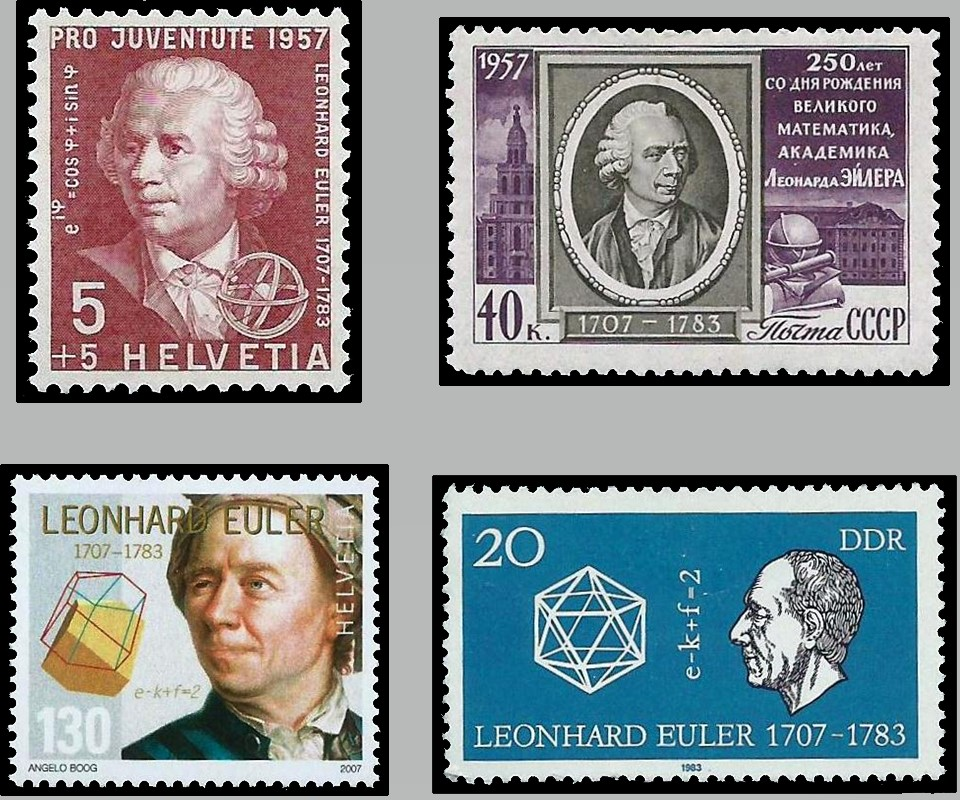
\includegraphics[scale=0.4]{img/euler.eps}
 \captionsetup{labelformat=empty}
 \caption{各国发行的欧拉纪念邮票。欧拉(Leonhard Euler)1707 - 1783}
 \label{fig:Arithmetica}
\end{figure}
%\end{wrapfigure}

1727年,欧拉成为俄罗斯圣彼得堡科学院的成员。他以旺盛的精力投入研究,在俄国的14年中,他在分析学、数论和力学方面作了大量出色的工作。1741年受腓特烈大帝的邀请到柏林科学院工作,达25年之久。在柏林期间他的研究内容更加广泛,涉及行星运动、刚体运动、热力学、弹道学、人口学,这些工作和他的数学研究相互推动。欧拉这个时期在微分方程、曲面微分几何以及其他数学领域的研究都是开创性的。1766年,叶卡捷琳娜二世在位期间,欧拉应邀重新返回圣彼得堡,并在那里直到逝世。

欧拉渊博的知识,无穷无尽的创作精力和空前丰富的著作,都是令人惊叹不已的。他从19岁开始发表论文,直到76岁,半个多世纪写下了浩如烟海的书籍和论文。几乎每一个数学领域都可以看到欧拉的名字。欧拉是科学史上最多产的一位杰出的数学家,一生发表论文共计856篇,专著31部。这还不包括1771年圣彼得堡火灾中失去的一部分。(欧拉的记录直到20世纪才由匈牙利数学家保罗·埃尔德什打破。后者发表的论文1525篇,著作32部。\cite{Wiki-Euler})

欧拉具有超出常人的坚强意志。1735年,他的右眼开始失明。1771年原本正常的左眼也完全失明了。正如失聪没有阻止贝多芬的音乐创作一样,失明也同样没有阻止欧拉的数学探索\cite{HanXueTao2009}。在书记员的帮助下,欧拉在多个领域的研究其实变得更加高产了。在1775年,他平均每周就完成一篇数学论文。欧拉一生中有一半著作都是在双目完全失明后口述完成的。欧拉的多产并不是偶然的,他有着惊人的记忆力。不但能够记住前100个素数,而且还能记住它们的平方、立方甚至更高次方。他还可以进行复杂的心算。法国物理学家阿拉戈(François Arago)说“欧拉计算时就像人在呼吸、鹰在翱翔一样轻松”。欧拉可以在任何不良的环境中工作,他常常抱着孩子在膝上完成论文,也不顾孩子在旁边喧哗。

欧拉的著作中既有难度很高的专著,也有专为普通大众所写的读物。他还特意为青少年写过一本书——《给德国公主的信》。并为非数学专业的读者写了一本初等代数教程,这本书至今仍在印刷。欧拉特别重视表达的清晰易懂。我们今天很多熟知的数学符号,都是欧拉精心选用的,例如$\pi$(1736年),虚数单位$i$(1777年),$e$(1748年),三角函数$sin$和$cos$(1748年),$tg$(1753年),$\Delta x$(1755年),求和$\sum$(1755年),表示函数的$f(x)$(1734年)等\cite{HanXueTao2009}。

1783年9月18日,欧拉与朋友们吃饭。那天天王星刚发现不久,欧拉列出计算天王星轨道的要领。晚餐后,欧拉一边喝着茶,一边和小孙女玩耍,突然之间,烟斗从他手中掉了下来。他说了一声:“我的烟斗”,并弯腰去捡,结果再也没有站起来,他喃喃地说了一句:“我死了……”就这样“停止了计算和生命”\footnote{法国数学家孔多塞语}。

\vspace{5mm}

\index{RSA算法}
今天,费马小定理已经走进人们的日常生活中,不管是网络购物还是电子交易。1976年,美国斯坦福大学的教授马丁$\cdot$赫尔曼(Martin Hellman)和惠特菲尔德$\cdot$迪菲(Whitfield Diffie)提出了非对称公钥加密算法的思想。1977年美国麻省理工学院的罗纳德$\cdot$李维斯特(Ron Rivest)、阿迪$\cdot$萨莫尔(Adi Shamir)和伦纳德$\cdot$阿德曼(Len Adleman)提出了构造单向函数的数论方法,从而产生了以这三个人姓氏首字母命名的RSA算法。

RSA算法的核心思想是人们可以容易地将两个大素数乘在一起得到一个合数,然而在不事先知道这两个素数的情况下,对这个合数做因数分解却非常困难。对于一个200位以上的的大数做因式分解,即使用强大的超级计算机,所耗费的时间也要超过宇宙的年龄。因此,如果能够迅速地找到大素数,就可以构造难以破解的密钥。但是素数的存在规律是神秘的,人们没有找到素数的“通项公式”。最原始的办法是挑选一个数$n$,然后逐一验证从1到$\sqrt{n}$之间的整数能否整除$n$。但这种方法非常低效,对大数进行素数检测,同样会超过宇宙年龄所需的时间。稍好的方法是埃拉托斯特尼筛法。列出从2开始到$n$之间的整数,然后从2开始,先筛除所有2的倍数,然后再筛除3的倍数,这样每次都从没有被筛除的第一个数开始重复这一步骤,直到把不大于$\sqrt{n}$的所有倍数都筛除为止。这样就可以获得$n$以内的所有素数。但这样方法同样只是对较小的整数$n$有效。无法达到大素数检测的目的。

费马小定理恰好给出了一种大素数检验的办法。对于一个大整数$n$,我们可以随机挑选一个小于$n$的正整数$a$,将其称为“证人”(witness),然后检查$a^{n-1}$模$n$的余数是否等于1,如果不是1,根据费马小定理,$n$一定不是素数。如果等于1,则$n$有可能是素数。

根据这一思想构造的“费马素数检测”算法如下:

\begin{algorithmic}
\Function{primality}{$n$}
  \State 随机选择正整数$a < n$
  \If{$a^{n-1} \equiv 1 \mod n$}
    \State \Return 素数
  \Else
    \State \Return 合数
  \EndIf
\EndFunction
\end{algorithmic}

我们并不需要真的计算$a$的$n-1$次方然后再求除$n$的余数,而是通过模乘运算。并且还可以进一步利用中间的计算结果加速,例如当我们得到$b = a^2 \mod n$时,可以直接计算$b^2 \mod n$从而得到$a^4 \mod n$。假设要计算$a^{11} \mod n$,因为:

\[
a^{11} = a^{8 + 2 + 1} = ((a^2)^2)^2a^2a \mod n
\]

所以我们真正需要计算的只有$a^2 \mod n$, $(a^2)^2 \mod n$, $((a^2)^2)^2 \mod n$。为此,我们可以把$n$表示为2进制,然后仅仅迭代计算数字为1所在位上的模乘结果,这是一个复杂度为$O(\lg n)$的算法。因此费马素数检测的速度很快。

但某个数即使通过了费马素数检测,仍然不一定是素数,例如341 = 11 $\times$ 31,但是$2^{340} \equiv 1 \mod 341$。为了减少费马检验的“假阳性”,人们进行了一系列改进。首先是适当增加证人的数量。人们发现,如果一个数无法通过费马检验,那么至少存在一半小于$n$的数都无法通过费马检验\cite{Algorithms-DPV}(26页)。

\begin{theorem}
正整数$a$小于$n$,且和$n$互素,如果$a^{n-1} \not\equiv 1 \mod n$,则所有$a<n$的选择中,至少有一半也是这样。
\end{theorem}

\begin{figure}[htbp]
\centering
\begin{tikzpicture}[scale=0.8]
\draw (0, 0) circle[x radius=1cm, y radius=3cm]
      (5, 0) circle[x radius=1cm, y radius=3cm];
\path (0, 3) node[above] {通过费马测试的数}
      (5, 3) node[above] {未通过费马测试};
\path (0, 0) node (b) {}
      (5, 0) node (fb) {}
      (0, 1.5) node (a) {}
      (5, 1.5) node (fa) {}
      (0, -1.5) node (c) {}
      (5, -1.5) node (fc) {};
\filldraw (0, 0) circle (1pt) node[above] {}
      (5, 0) circle (1pt) node[above] {}
      (0, 1.5) circle (1pt) node[above] {$b$}
      (5, 1.5) circle (1pt) node[above] {$ab$}
      (5, 1) circle (1pt) node[right] {$c$}
      (0, -1.5) circle (1pt) node[above] {}
      (5, -1.5) circle (1pt) node[above] {};
\draw[dashed, ->] (b) to node [above] {$f: b \to ab$} (fb)
      (a) to [bend left] (fa)
      (c) to [bend right] (fc);
\end{tikzpicture} \\
集合$\{1, 2, ..., n-1\}$
\caption{从通过费马测试的集合向未通过的集合做映射}
\label{fig:Fermat-test}
\end{figure}

\begin{proof}
若某个$a$使得$a^{n-1} \not\equiv 1 \mod n$,对于任何可以同行过费马检测的证人$b$(即$b^{n-1} \equiv 1 \mod n$),都可以构造一个费马检测的反例$ab$

\[
(ab)^{n-1} \equiv a^{n-1}b^{n-1} \equiv a^{n-1}1 \not\equiv 1 \mod n
\]

并且,由于$i \neq j$,有$a \cdot i \not\equiv a \cdot j$,所以这些反例都是彼此不同的。

如图\ref{fig:Fermat-test}所示,如果存在不通过费马测试的整数,则这样的数至少和通过的一样多。
\end{proof}

为此,我们可以多次选取不同的证人$k$次执行费马检验,这样就可以把$n$不是素数的概率降低到$\dfrac{1}{2^k}$。但实际上存在这样的合数$n$,使得任何小于$n$且和$n$互素的数$a$都有$a^{n-1} \mod n$。也就是说无论选什么样的$a$,这样的合数都能通过费马检测。卡迈克尔(Carmichael )在1910年发现了第一个这样的数561 = 3 $\times$ 11 $\times$ 17,这样的数现在被称为卡迈克尔数,或者费马伪素数\footnote{捷克数学家西摩尔卡(Václav Šimerka)在1885年发现了前7个费马伪素数:561 = 3 $\times$7 $\times$11, 1105 = 5 $\times$13 $\times$7, 1729 = 7 $\times$13 $\times$19, 2465 = 5 $\times$17 $\times$29, 2821 = 7 $\times$13 $\times$31, 6601 = 7 $\times$23 $\times$41, 8911 = 7 $\times$19 $\times$67。但是他的工作不为人知。}。埃尔德什曾经猜测有无穷多个卡迈克尔数,1994年人们证明了对足够大的$n$,在1到$n$之间至少存在$n^{2/7}$个卡迈克尔数。从而说明存在无穷多的卡迈克尔数\cite{Wiki-Carmichael-number}。

实际的RSA算法采用“米勒——拉宾”进行素数测试。它也是一种概率算法\footnote{米勒——拉宾素数检验存在一个确定性算法的版本,但是其正确性依赖于黎曼假设(黎曼猜想)\cite{Wiki-Miller-Rabin}。}。根据上述定理,如果选择超过100个证人,错误率会低于$\frac{1}{2^{100}}$。高德纳说:“该测试的错误率要比计算机因为宇宙辐射而丢失某个二进制位的概率还要低。”
%读着可以参考本书的附录,了解RSA算法的详细原理和实现。

\vspace{5mm}

到目前为止,我们介绍过的群、半群、幺半群的关系总结如下。

\begin{figure}[htbp]
\centering
\begin{tikzpicture}[scale=0.8]
\draw (4, 2) node (abeliangroup) {阿贝尔群}
      (2, 1) node (group) {群}
      (0, 0) node (monoid) {幺半群}
      (-2, -1) node (semigroup) {半群};
\draw (-4, -2) circle[x radius = 1.5cm, y radius = 0.5cm] node (assoc) {结合性}
      (0, -2) circle[x radius = 1.5cm, y radius = 0.5cm] node (binop) {二元运算}
      (2, -1) circle[x radius = 1.5cm, y radius = 0.5cm] node (unit) {单位元}
      (4, 0) circle[x radius = 1.5cm, y radius = 0.5cm] node (invert) {可逆性}
      (6, 1) circle[x radius = 1.5cm, y radius = 0.5cm] node (community) {交换性};
\draw (abeliangroup) to (community)
      (abeliangroup) to (group)
      (group) to (invert)
      (group) to (monoid)
      (monoid) to (unit)
      (monoid) to (semigroup)
      (semigroup) to (binop)
      (semigroup) to (assoc);
\end{tikzpicture}
\caption{群、半群、幺半群}
\label{fig:groups}
\end{figure}

\begin{Exercise}
\Question{今天是星期日,$2^{100}$天以后是星期几?}
\Question{任给两个串(字符串或者列表),如何通过编程判断它们可以连成相同的项链?}
\Question{编程实现埃拉托斯特尼筛法。}
\Question{利用埃拉托斯特尼筛法的思想,编程产生2到100内正整数的欧拉$\upphi$函数表。}
\Question{编程实现模乘的幂运算,并实现费马素数检测。}
\end{Exercise}

\section{环与域}

\begin{wrapfigure}{R}{0.3\textwidth}
%\begin{figure}[htbp]
 \centering
 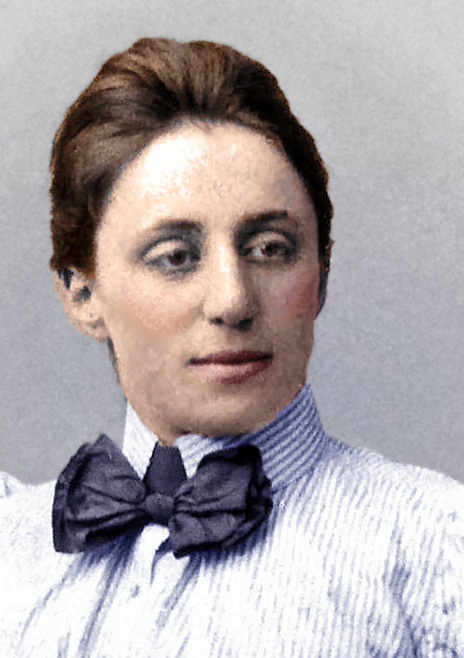
\includegraphics[scale=1]{img/Noether.eps}
 \captionsetup{labelformat=empty}
 \caption{埃米$\cdot$诺特 1882-1935}
 \label{fig:Arithmetica}
%\end{figure}
\end{wrapfigure}

\index{诺特(Emmy Noether)}
现代抽象数学中环和域的概念是由德国女数学家埃米$\cdot$诺特所发展的。1882年3月23日,诺特生于德国大学城埃尔朗根的一个犹太人家庭。她的父亲是埃尔朗根大学的数学家。诺特本来打算将来教授法文和英文,但在父亲的影响下,她逐渐对数学产生了兴趣。1900年冬天,18岁的诺特考进了爱尔朗根大学。当时,大学里不允许女生注册,女生顶多只有自费旁听的资格。大学的几百名学生中只有两名女生,诺特大大方方地坐在教室前排,认真听课,刻苦学习,后来,她勤奋好学的精神感动了主讲教授,破例允许她与男生一样参加考试。1903年7月,诺特顺利通过了毕业考试,男生们都取得了文凭,而她却成了没有文凭的大学毕业生。诺特生活在公开歧视妇女发挥数学才能的制度下。毕业以后她在埃尔朗根数学研究院工作,长达7年却没有任何工资。1907年12月,她以优异的成绩通过了博士考试,成为第一位女数学博士。此后,她在著名的数学家高丹、费叶尔的指引下,在数学的不变式领域进行了深入的研究。1915年,应著名数学家希尔伯特和克莱因的邀请,诺特来到数学圣地哥廷根大学。不久,她就以希尔伯特教授的名义,在哥廷根大学讲授数学课程。希尔伯特十分欣赏诺特的才能,想帮她在哥廷根大学找一份正式的工作。当时的哥廷根大学没有专门的数学系,数学、语言学、历史学都划在哲学系里,聘请必须经过哲学教授会议批准。希尔伯特的努力遭到教授会议中语言学家和历史学家的极力反对,他们出于对妇女的传统偏见,连聘为“私人讲师”这样的请求也断然拒绝。希尔伯特屡次据理力争都没有结果,他在一次教授会上愤愤地说:“我简直无法想象候选人的性别竟成了反对她升任讲师的理由。先生们,别忘了这里是大学而不是洗澡堂!”

在希尔伯特等人的影响下,不到两年时间,诺特就发表了两篇重要论文。诺特为爱因斯坦的广义相对论给出了一种纯数学的严格方法。并提出了现代物理学中称为“诺特定理”的观点。就这样,诺特以她出色的科学成就,迫使那些歧视妇女的人也不得不于 1919年准许她升任讲师。此后,诺特走上了完全独立的数学道路。1921年,她从不同领域的相似现象出发,把不同的对象加以抽象化、公理化,然后用统一的方法加以处理,完成了《环中的理想论》这篇重要论文。这是一项非常了不起的数学创造,它标志着抽象代数学真正成为一门数学分支,或者说标志着这门数学分支现代化的开端。诺特也因此获得了极大的声誉,被誉为是“现代数学代数化的伟大先行者”,“抽象代数之母”。1931年,她的学生荷兰数学家的范德瓦尔登系统总结了整个诺特学派的成就,出版了《近世代数》一书,影响了许多当时的青年数学家。1932年,诺特的科学声誉达到了顶点。在这一年于苏黎世举行的第9届国际数学家大会上,诺特作了长达1小时的大会发言,受到广泛的赞扬。

然而,巨大的声誉并未改善诺特的艰难处境。在不合理的制度下,灾难和歧视像影子一样缠住了她。1922年,由于大数学家希尔伯特等人的推荐,诺特终于在清一色的男子世界——哥廷根大学取得教授称号。不过,那只是一种编外教授,没有正式工资,于是,这位历史上最伟大的女数学家,只能从学生的学费中支取一点点薪金,来维持极其简朴的生活。希特勒上台后,德国法西斯对犹太人的迫害愈演愈烈。1929年,诺特被撵出居住的公寓。1933年4月,法西斯当局剥夺了诺特教书的权利,将一批犹太人教授逐出校园,诺特只好辗转逃往美国。尽管她是世界知名的数学家,但由于是女性,诺特没有获得大型研究院校的聘约。最后,她在一家名为布林莫尔(Bryn Mawr)的女校以访问学者的身份任教。1935年,诺特做了卵巢囊肿摘除手术,4月14日不幸去世,终年53岁。

诺特善于通过透彻的洞察建立优雅的抽象概念,再将之漂亮地形式化。被帕维尔·亚历山德罗夫、爱因斯坦、迪厄多内、外尔和维纳形容为数学史上最重要的女性。她彻底改变了环、域和代数的理论。在物理学方面,诺特定理解释了对称性和守恒定律之间的根本联系,她还被称为“现代数学之母”,她允许学者们无条件地使用她的工作成果,也因此被人们尊称为“当代数学文章的合著者”\cite{Wiki-Noether}。

\subsection{环的定义}
\index{环}
我们接下来看一看环(ring)的定义。

\begin{definition}
一个集合$R$叫做一个环,如果满足以下条件:
\begin{enumerate}
\item $R$是一个加群,也就是说$R$对于其上定义的某种加法构成一个阿贝尔群;
\item $R$上还定义了乘法,并且对于这个乘法是封闭的;
\item 乘法满足结合律,任意$a, b, c$,有:$(ab)c = a(bc)$;
\item 满足分配律,任意$a, b, c$都有:
\[
\begin{array}{l}
a(b + c) = ab + ac \\
(b + c)a = ba + ca
\end{array}
\]
\end{enumerate}
\end{definition}

\index{交换环}
显然,全体整数对于普通加法和乘法构成一个环。另外多项式和矩阵对于加法和乘法也构成一个环。在环的定义中,我们只要求加法满足交换律,构成阿贝尔群。而对乘法没有要求。如果乘法也适合交换律,我们称这样的环为\textbf{交换环}。在一个交换环里,对于正整数$n$和任何两个元都有:

\[
a^nb^n = (ab)^n
\]

在环的定义中,我们也没有要求环中的乘法一定要有单位元。如果$R$中存在一个元素$e$的,使得对任何元素都有:

\[
ea = ae = a
\]

则称$e$为环的单位元。一般来说,一个环未必有单位元。习惯上我们常用1来代表单位元,当然这只是一个符号,它并不是数字1。有了单位元,自然也可以规定逆元。如果$ab = ba = 1$,我们称$b$是$a$的逆元。从群的性质我们可以推知,如果一个环有单位元,这个单位元必然是唯一的。如果一个元素有逆元,这个逆元也必然是唯一的。但是并非任何元素都逆元,例如整数环有单位元,但除了$\pm 1$外,其它整数都没有逆元。

由于环上有结合律,所以我们有:

\[
(a - a)a = aa - aa = 0
\]

也就是说,如果$a$或$b$中有一个是0,则$ab = 0$。但是这一结论的逆命题却不成立。也就是说,由$ab = 0$,并不能推知$a$或$b$中存在一个0。我们来看一个反例。考虑模$n$的剩余类,其中加法是模$n$的加法:$[a] + [b] = [a + b]$,即相加后对$n$取模,其构成一个交换加群。模$n$的乘法定义为:$[a][b] = [ab]$,即相乘后对$n$取模。容易验证这构成一个环,称为模$n$的剩余类环。

如果$n$不是素数,例如10,我们发现两个非0元素$[5][2] = [5 \times 2] = [0]$。事实上,把$n$分解成两个因子,其模乘的结果必然是零。

\index{零因子}
在一个环里,如果$a \neq 0, b \neq 0$,但却有$ab = 0$,我们说$a$是环的一个\textbf{左零因子},$b$是环的一个\textbf{右零因子}。如果环是交换环,那么一个左零因子同时也是右零因子。当然,一个环可能没有零因子,例如整数环。只有在不存在零因子的环里,我们才能从$ab = 0$推知$a$或$b$等于0。并且我们有如下定理:

\begin{theorem}
一个没有零因子的环里,以下两个消去律都成立:
\begin{itemize}
\item 若$a \neq 0$,$ab = ac$,则$b = c$;
\item 若$a \neq 0$,$ba = ca$,则$b = c$;
\end{itemize}
\end{theorem}

反之,如果一个环里任一个消去律成立,则另一个也必然成立,并且环中没有零因子。

\index{整环}
这样,我们认识了一个环的三种附加条件:一是乘法满足交换律;二是单位元存在;三是不存在零因子。同时满足这三个附加条件的环有一个特殊名称,叫做\textbf{整环}(integral domain)。整数环显然是一个整环。

\index{半环}
有些情况下,环的条件太强了。我们并不需要加法一定存在逆元(即加法取反,additive inverse)。如果放宽条件,我们就得到\textbf{半环}这种代数结构。

\begin{definition}
一个集合$R$,以及其上定义的某种加法和乘法称作半环,如果它满足以下条件。
\begin{enumerate}
\item $R$上的加法构成一个交换幺半群,并且存在一个称为0的单位元;
\item $R$上的乘法构成了一个幺半群,并且存在一个称为1的单位元;
\item 满足分配律,任意$a, b, c$都有:
\[
\begin{array}{l}
a(b + c) = ab + ac \\
(b + c)a = ba + ca
\end{array}
\]
\item 0元乘以任何元都得0。即$a0 = 0a = 0$
\end{enumerate}
\end{definition}
自然数$N$就是半环的典型例子。布尔运算是一个只有两个元素的半环。

\begin{Exercise}
\Question{证明本节的定理,一个没有零因子的环里,两个消去律成立。}
\Question{证明所有形如$a + b \sqrt{2}$,其中$a, b$是整数的实数对于普通加法和乘法构成一个整环。}
\end{Exercise}

\subsection{除环和域}

我们知道一个环里不一定所有的元素都有逆元。如果某个环中所有的元素都有逆元,就构成一种特殊的环。例如全体有理数对于普通加法和乘法来说显然是一个环,这个环中任意不等于零的元$a$都有逆元$\frac{1}{a}$。

\index{除环}
\begin{definition}
一个环$R$如果满足以下条件,则叫做\textbf{除环}:
\begin{enumerate}
\item $R$至少包含一个不等于零的元;
\item $R$有一个单位元;
\item $R$的每个不等于零的元都有一个逆元。
\end{enumerate}
\end{definition}

\index{域}
\begin{definition}
一个交换除环叫做一个\textbf{域}。
\end{definition}

按照这一定义,全体有理数构成一个域。同样,全体实数或者全体复数的集合对于普通加法和乘法也各自构成一个域\footnote{我们在后面章节会看到,有理数域是可数的,而实数、复数域是不可数的}。除环和域有一些有趣的性质。一个除环没有零因子。这是因为,如果$a \neq 0$,并且$ab = 0$。我们在两边左乘$a$的逆元:

\[
a^{-1}ab = b = 0
\]

这样必然有$b$等于零,所以除环不含有零因子。第二个性质是,一个除环中的所有非零元,对于乘法构成一个群$R*$,我们称$R*$叫做除环$R$的乘群。这样一个除环是由两个群:加群与乘群组合而成的;分配率好像是一座桥梁,使得两个群发生联系。到目前为止,我们介绍过的环、半环、整环、除环和域的关系总结如图\ref{fig:ring}。

\begin{figure}[htbp]
\centering
\begin{tikzpicture}[scale=0.8]
\draw (0, 1) node (semiring) {半环}
      (0, 0) node (ring) {环}
      (-4, -1) node (commu-ring) {交换环}
      (0, -1) node (unit) {有单位元}
      (3, -1) node (zero-factor) {无零因子}
      (-3, -3) node (integral-domain) {整环}
      (3, -3) node (division-ring) {除环}
      (0, -4) node (field) {域};
\draw (0, 2) circle[x radius = 1.5cm, y radius = 0.5cm] node (add-monoid) {加法幺半群}
      (4, 2) circle[x radius = 1.5cm, y radius = 0.5cm] node (mul-monoid) {乘法幺半群}
      (-4, 2) circle[x radius = 1.5cm, y radius = 0.5cm] node (distribution-law) {分配律}
      (4, 0.5) circle[x radius = 1.5cm, y radius = 0.5cm] node (negate) {加法可求反}
      (-5, 0) circle[x radius = 1.5cm, y radius = 0.5cm] node (mul-commu) {乘法可交换}
      (0, -3) circle[x radius = 1.5cm, y radius = 0.5cm] node (mul-invert) {乘法可求逆};
\draw (distribution-law) to (semiring)
      (add-monoid) to (semiring)
      (mul-monoid) to (semiring)
      (semiring) to (ring)
      (negate) to (ring)
      (mul-commu) to (commu-ring)
      (ring) to (commu-ring)
      (ring) to (unit)
      (ring) to (zero-factor)
      (commu-ring) to (integral-domain)
      (unit) to (integral-domain)
      (zero-factor) to (integral-domain)
      (unit) to (division-ring)
      (zero-factor) to (division-ring)
      (integral-domain) to (field)
      (division-ring) to (field)
      (mul-invert) to (division-ring);
\end{tikzpicture}
\caption{半环、环、整环和域}
\label{fig:ring}
\end{figure}

还有一些重要的概念,如子环、理想、主理想环与欧几里得环限于篇幅我们不在这里介绍了。

\section{伽罗瓦理论}
我们分别介绍了域和群,而伽罗瓦理论像是一座桥梁把它们连接到了一起。域里面有加减乘除四种运算和无穷多个元素,是很复杂的对象。而伽罗瓦理论可以把域中的一些问题化简到只有一种运算的有限群里去。整个伽罗瓦理论的核心思想就是这一点。

伽罗瓦理论无疑是相当艰深难懂的。今天我们读到的伽罗瓦理论不再模糊费解,而是经过不下二十位大师的发展和处理的。其中最主要的贡献当属若当、戴德金和阿廷。若当和戴德金分别在法国和德国最早系统地整理伽罗瓦理论。今天使用的伽罗瓦群的定义是由戴德金给出的。阿廷使得伽罗瓦理论取得了现代的形式\cite{ZhangPu2013}。为了在这么短的一个章节介绍伽罗瓦理论,我采用了对初学者比较容易理解的一种解释\cite{Stillwell1994}。对于一般的读者,可能仍然无法一遍就弄懂它。开卷有益,生活不是线性发展的。我建议大家不断回过头去重温此前介绍的一些概念,并阅读那些名著。每次也许有不同的体会,让我们一起享受那种一览众山小的感觉。

\subsection{扩域}
\index{扩域}
根据域的定义,我们知道全体有理数构成一个域,记作$Q$。我们现在考虑所有形如$a + b\sqrt{2}$的数组成的集合,其中$a, b$都是有理数\cite{Goodman2011}。显然有理数是这一集合的子集(只要让$b=0$即可)。容易验证,任何两个这样的数做加、减、乘法都仍然可以写成$a + b \sqrt{2}$的形式。除法稍微难些。观察$x = \dfrac{1}{a + b\sqrt{2}}$,我们可以将分子分母同时乘以$a - b \sqrt{2}$,这样就有:

\[
\begin{array}{rl}
x & = \dfrac{a - b \sqrt{2}}{(a + b \sqrt{2})(a - b \sqrt{2})} \\[2ex]
  & = \dfrac{a - b \sqrt{2}}{a^2 - 2b^2}
\end{array}
\]

令$p = a^2 - 2b^2$,这样$x$就可以表示成$(a/p) -(b/p)\sqrt{2}$。这样除法也就验证了。的的确确这一集合构成一个域。我们将其记为$Q[\sqrt{2}]$。同理$Q[\sqrt{3}]$也是一个域。这就引出了扩域的概念。

\begin{definition}
如果域$E$包含域$F$,我们称$E$是$F$的\textbf{扩域},记作$F \subseteq E$或者$E/F$。
\end{definition}

例如实数域就是有理数域的扩域,$Q[\sqrt{2}]$是有理数域$Q$的扩域。一般来说,如果$F$是一个域,$\alpha \in F$,但是$\sqrt{\alpha} \not\in F$,则$F_1 = F[\sqrt{\alpha}]$仍是一个域。这样,我们就可以重复使用这个方法不断扩张。若$\beta \in F_1$, 但$\sqrt{\beta} \not\in F_1$,则:

\[
\begin{array}{rl}
F_2 & = F_1[\sqrt{\beta}] \\
    & = F[\sqrt{\alpha}][\sqrt{\beta}] \\
    & = F[\sqrt{\alpha}, \sqrt{\beta}]
\end{array}
\]

即所有形如$a + b \sqrt{\beta}$的数,其中$a, b \in F_1$的数构成了更高层次的扩域。这样我们就可以从有理数域开始,得到一个扩域系列:$Q \subset F_1 \subset F_2 ... \subset F_n$。

扩域有何意义呢?举个例子,方程$x^2 - 2 = 0$在有理数域上无解,但是它在有理数域的扩域$Q[\sqrt{2}]$上有一对解($x = \pm \sqrt{2}$)。我们进一步再看一个例子,方程$x^4 - 5x^2 + 6 = 0$在有理数域上无解,在扩域$Q[\sqrt{2}]$上有两个解$\pm \sqrt{2}$,在扩域$Q[\sqrt{2}, \sqrt{3}]$上有全部四个解$\pm \sqrt{2}, \pm \sqrt{3}$。于是就自然引出了根域的重要概念:

\index{分裂域} \index{根域}
\begin{definition}
包含方程$p(x) = 0$全部根的最小扩域叫做$p(x)$的\textbf{分裂域}。也称为根域。
\end{definition}

这样方程$x^2 -2 = 0$的分裂域就是$Q[\sqrt{2}]$。为什么叫做“分裂”呢?多项式$x^2-2$在有理数域$Q$上是不可约的,但是在扩域$Q[\sqrt{2}]$上可以“分裂”成:
\[
(x + \sqrt{2}) (x - \sqrt{2})
\]
对于某一多项式方程,如果我们能够从基本域有理数域开始,通过一系列上述的扩域,最终到达分裂域,那么自然这个方程是可以用根式解的。

我们给出了平方根的例子,显然还有更加复杂的情况。3次方程可能要开3次方根,有些方程甚至还需要虚数单位$i$。从高中数学我们知道,最简单的方程$x^p-1=0$含有$p$个根$1, \zeta, \zeta^2, ..., \zeta^{p-1}$,其中$\zeta \neq 1$是单位圆上的一个复根。为了涵盖这些情况,我们需要更加严格地描述扩域。

\begin{figure}[htbp]
\centering
\begin{tikzpicture}[scale=3]
 \draw[step=.5cm, gray, very thin] (-1.2,-1.2) grid (1.2,1.2);
 \draw[->] (-1.25,0) -- (1.25,0) coordinate (x axis);
 \draw[->] (0,-1.25) -- (0,1.25) coordinate (y axis);
 \draw (0,0) circle (1cm);
 \draw[->, very thick] (0, 0) edge node[below=2pt,fill=white] {$\zeta^0 = \zeta^3 = 1$} (1, 0)
     (0, 0) edge node[above] {$\zeta = \dfrac{-1 + i\sqrt{3}}{2}$} (120:1cm)
     (0, 0) edge node[below] {$\zeta^2 = \dfrac{-1 - i\sqrt{3}}{2}$} (-120:1cm);
\end{tikzpicture}
\caption{单位根,$x^3 - 1 = 0$}
\label{fig:root-of-unity}
\end{figure}

如果$\alpha$的整数次方等于域$F$中的某个元素$b$,也就是说$\alpha^m = b \in F$,这样$\alpha$就可以写成$b$的根式形式$\alpha = \sqrt[m]{b}$。我们可以逐一用这样的一组根式进行扩域,从而得到$F[\alpha_1][\alpha_2]...[\alpha_k]$。如果每次扩张所用的$\alpha_i$都是根式,我们称扩域$F[\alpha_1, \alpha_2, ..., \alpha_k]$为$F$的根式扩域(radical extension)。设方程的根是$x_1, x_2, ..., x_n$(注意,这里我们没有说$x_i$一定是根式),如果其分裂域$E = Q[x_1, x_2, ..., x_n]$是根式扩域,我们说方程是根式可解的。

\begin{Exercise}
\Question{证明$Q[a, b] = Q[a][b]$,其中$Q[a, b]$是所有由$a, b$组成的表达式如$2ab, a + a^2b$等。}
\end{Exercise}

\subsection{自同构和伽罗瓦群}

到目前为止,我们的思路是从方程系数所在的有理数域开始,通过逐步根式扩域,向较高层次的分裂域前进。如何进一步化简难题,找到答案呢?伽罗瓦在此进行逆向思维。他转而去考虑方程根之间的对称性。例如方程$x^2 - 2 = 0$有一对根$\pm \sqrt{2}$。显然用$-\sqrt{2}$去代替$\sqrt{2}$,方程仍然成立。除此之外,将等式$\sqrt{2}^2 + \sqrt{2} + 1 = 3 + \sqrt{2}$中的$\sqrt{2}$替换成$-\sqrt{2}$也是成立的。也就是说,这对根$\pm \sqrt{2}$,对于关系$\alpha^2 + \alpha + 1 = 3\alpha$是对称的。进一步说,对于任何仅仅对$\sqrt{2}$进行乘法和加法的表达式,这对根都可以进行互换。今天我们知道,描述对称的最有力武器是群。具体说是置换群(如果记不清了,请回过头去再看一下\ref{symmetric group})。于是伽罗瓦引入了域上的自同构概念,将扩域和群联系了起来。

我们还是用$Q[\sqrt{2}]$举例子。如果我们定义一个从$Q[\sqrt{2}]$到$Q[\sqrt{2}]$的函数$f: Q[\sqrt{2}] \to Q[\sqrt{2}]$。它的具体定义为:
\[
f(a + b \sqrt{2}) = a - b \sqrt{2}
\]

则$f$就是一个域上的自同构。

\index{自同构}
\begin{definition}
\textbf{域的自同构}(Field Automorphism)是一个可逆函数$f$,它满足$f(x + y) = f(x) + f(y)$,$f(ax) = f(a) f(x)$,$f(1/x) = 1/f(x)$。
\end{definition}

我们可以验证,前面那个例子$f(a + b \sqrt{2}) = a - b \sqrt{2}$满足这三个条件。域的自同构背后的思想是,我们可以重新调换域中的元素,而完全不影响域的结构。

\begin{definition}
$F$-自同构:进一步,如果$E$是$F$的扩域,并且在域$E$的自同构$f$的基础上还满足一条额外的性质:对$F$中的任何元素$x$都有$f(x) = x$,则称为$E$上的$F$-自同构。
\end{definition}

这样就非常精确地定义了根的对称性。$F$-自同构对$F$中的所有元素都原样保持不动,而仅仅调换扩域$E$中新元素。对域中的元素进行调换恰好是置换(permutation)的思想,置换后保持不变恰好是对称的概念。对于$Q[\sqrt{2}]$这个例子,只有两个$Q$-自同构:一个是恒等变换$g(x) = x$,另外一个就是我们前面定义的$f$。

现在我们把目前得到的结果用例子$p(x) = x^2 - 2$总结一下:

\begin{enumerate}
\item $p(x)$的分裂域是$Q[\sqrt{2}]$;
\item $p(x)$的$Q$-自同构代表了根的对称性,它包含两个变换:$f(a + b\sqrt{2}) = a - b\sqrt{2}$和$g(x) = x$。
\end{enumerate}

但是仅仅扩展到分裂域并不能保证对所有的根完全对称。例如$x^4 - 5x + 6 = 0$的分裂域是$Q[\sqrt{2}, \sqrt{3}]$,虽然我们有能够调换$\pm \sqrt{2}$的自同构$f$,但是不存在能够调换$\sqrt{2}$和$\sqrt{3}$的自同构。否则根据自同构的定义$f(x) = x$,如果$f(\sqrt{2}) = \sqrt{3}$,则$f(\sqrt{2})^2 = \sqrt{3}^2$,即$\sqrt{2} = \sqrt{3}$。这显然是错误的。另外,考虑根式扩域$Q[x_1, ..., x_n, \sqrt{x_1}]$,它包含$x_1$的平方根,但是不含$x_2$的平方根。因此不存在能够调换$x_1$和$x_2$的自同构。为了恢复对称性,我们可以继续把$\sqrt{x_2}, ..., \sqrt{x_n}$扩展到域里。

\begin{theorem}
对于每个$Q[x_1, ..., x_n]$的根式扩域$E$,都存在一个更大的根式扩域$E \subseteq \overline{E}$,使得所有$x_1, ..., x_n$的置换都有自同构$\sigma$。
\end{theorem}

至此,我们已经把扩域和自同构联系了起来。如果把所有的自同构做成一个集合,这些自同构间的二元运算是复合(composite)变换,恒等变换是单位元,我们就得到了一个群。这个群被称作伽罗瓦群。

\index{伽罗瓦群}
\begin{definition}
\textbf{伽罗瓦群}:对于$F$的扩域$E$,我们有一组$E$的$F$-自同构的集合$G$。对任意$G$中的两个$F$-自同构$f, g$,定义二元运算$(f \cdot g)(x) = f(g(x))$。我们称$G$为扩域$E/F$的伽罗瓦群。记为$Gal(E/F)$。
\end{definition}

我们还是用$p(x) = x^2 - 2$举例。伽罗瓦群$G = Gal(p) = \{f, g\}$,包含两个元素,一个是$f(a + b\sqrt{2}) = a - b\sqrt{2}$,另一个是$g(x) = x$。其中单位元是$g$。我们来验证是否有$f \cdot f = g$:

\[
\begin{array}{rll}
(f \cdot f)(a + b\sqrt{2}) & = f(f(a + b\sqrt{2})) & \text{群运算的定义} \\
  & = f(a - b\sqrt{2}) & \text{对内层括号用$f$的定义} \\
  & = a + b\sqrt{2} & \text{再次用$f$的定义} \\
  & = g(a + b\sqrt{2}) & \text{恒等变换$g$的定义}
\end{array}
\]

这说明$G$的确是一个群,并且在同构的意义下等同于二阶循环群,它也同构于二阶对称群$S_2$。这个群可以写成$\{f, f^2\}$,这是因为$f^2 = f \cdot f = 1$,是群的单位元。也可写成置换群的形式$\{(1), (1\ 2)\}$,其中(1)是保持两个根不变,(1 2)是对调两个根。

\begin{Exercise}
\Question{试证明:对于有理数系数的任何多项式$p(x)$,若$E/Q$是扩域,$f$是$E$上的$Q$-自同构,则有$f(p(x)) = p(f(x))$。}
\Question{考虑复数,多项式$p(x) = x^4-1$的分裂域是什么?它的$Q$-自同构中有哪些变换?}
\Question{尝试写出二次方程$x^2 - bx + c = 0$的伽罗瓦群。}
\Question{证明,如果$p$是素数,则方程$x^p - 1$的伽罗瓦群是$q-1$阶的循环群$C_{q-1}$。}
\end{Exercise}

\subsection{伽罗瓦基本定理}
\index{伽罗瓦基本定理}

现在我们进入了伽罗瓦理论的核心部分了。从方程系数所在的域$F$开始,我们可以进行一系列扩域一直到达分裂域$F \subset F_1 \subset F_2 ... \subset E$。对应的伽罗瓦群为$Gal(E/F)$。伽罗瓦发现,这个群的所有子群和这些中间域$F_1, F_2, ...$之间存在着反序的一一对应。

\begin{theorem}
\textbf{伽罗瓦基本定理}:令$E/F$为扩域\footnote{严格说,要求是伽罗瓦扩张,我们这里略去了伽罗瓦扩张的定义。},$G$是对应的伽罗瓦群。这个群的子群和中间域之间存在一一对应。若$F \subset L \subset E$,有$Gal(E/L) = H$,则$H$是$Gal(E/F)$的子群。
\end{theorem}

之所以说是反序,是因为,随着域的扩张,对应的群是减小的。扩张的起点是域$F$,此时对应的群是完整的伽罗瓦群$G = Gal(E/F)$;扩张的终点是分裂域$E$,此时的群只有一个元素,就是恒等变换$\{1\}$。扩张的中间域$L$,对应的群是$H = Gal(E/L)$,它是子群,有$Gal(E/L) \subset Gal(E/F)$。并且如果$H$是正规子群(如果记不清了,可回去看一下\ref{normal-subgroup}),则它的商群$G/H = Gal(L/F)$。

我们举一个具体的例子\cite{MArtin}(490页)。考虑方程$x^4 - 8x^2 + 15 = 0$,它也可以表示成$(x^2 - 3)(x^2 - 5) = 0$。它的系数域是有理数域$Q$,方程的分裂域是$E = Q[\sqrt{3}, \sqrt{5}]$。它的伽罗瓦群$Gal(E/Q)$的阶是4,同构于一个4阶循环群。可以找到3个中间扩域分别是$Q[\sqrt{3}]$, $Q[\sqrt{5}]$和$Q[\sqrt{15}]$,这3个中间扩域对应的子群的阶都是2。而方程的伽罗瓦群,也就是4阶循环群只有一个2阶子群。除此之外,它不再有其它非平凡子群了。根据伽罗瓦基本定理,我们知道,除了那3个中间扩域之外,再也没有其它中间扩域了。换个角度看,分裂域上的任何元素都可以表示为$\alpha = a + b\sqrt{3} + c\sqrt{5} + d\sqrt{15}$,其中$a, b, c, d$是有理数;对于3个中间扩域上的任何元素,$b, c, d$中至少有两个为0。

\begin{figure}[htbp]
\centering
\begin{tikzpicture}[scale=0.8]
\draw (-3, 3) node (Q3-5) {$Q[\sqrt{3}, \sqrt{5}]$}
      (-5, 0) node (Q5) {$Q[\sqrt{5}]$}
      (-3, 0) node (Q15) {$Q[\sqrt{15}]$}
      (-1, 0) node (Q3) {$Q[\sqrt{3}]$}
      (-3, -3) node (Q) {$Q$};
\draw (3, 3) node (G1) {$\{1\}$}
      (1, 0) node (G3) {$\{1, f\}$}
      (3, 0) node (G15) {$\{1, (f \cdot g)\}$}
      (5, 0) node (G5) {$\{1, g\}$}
      (3, -3) node (G) {$\{1, f, g, (f \cdot g)\}$};
\draw[->] (Q3-5) edge node[midway, above] {伽罗瓦群} (G1)
      (G) edge node[midway, above] {对应到扩域} (Q)
      (Q3) edge node[midway] {扩域} (Q3-5)
      (Q15) edge (Q3-5)
      (Q5) edge (Q3-5)
      (Q) edge (Q3)
      (Q) edge (Q15)
      (Q) edge (Q5)
      (G1) edge node[midway] {子群} (G3)
      (G1) edge (G15)
      (G1) edge (G5)
      (G3) edge (G)
      (G15) edge (G)
      (G5) edge (G);
\end{tikzpicture}
\caption{伽罗瓦对应}
\label{fig:Galois-Correspondence}
\end{figure}

如图\ref{fig:Galois-Correspondence}所示,分裂域上的任意元可以写成如下形式:

\[
\begin{array}{rl}
\alpha &= (a + b\sqrt{3}) + (c + d\sqrt{3}) \sqrt {5} \\
       &= a + b\sqrt{3} + c\sqrt{5} + d\sqrt{15}
\end{array}
\]

其中$a, b, c, d$都是有理数。我们定义如下自同构:

变换$f$将$\sqrt{3}$反号:

\[
\begin{array}{rl}
f((a + b\sqrt{3}) + (c + d\sqrt{3}) \sqrt {5} & = (a - b\sqrt{3}) + (c - d\sqrt{3})\sqrt{5} \\
 & = a - b\sqrt{3} + c\sqrt{5} - d\sqrt{15}
\end{array}
\]

变换$g$将$\sqrt{5}$反号

\[
\begin{array}{rl}
g((a + b\sqrt{3}) + (c + d\sqrt{3}) \sqrt {5} & = (a + b\sqrt{3}) - (c + d\sqrt{3})\sqrt{5} \\
 & = a + b\sqrt{3} - c\sqrt{5} - d\sqrt{15}
\end{array}
\]

复合变换$f \cdot g$同时将$\sqrt{3}$和$\sqrt{5}$反号

\[
\begin{array}{rl}
(f \cdot g)((a + b\sqrt{3}) + (c + d\sqrt{3}) \sqrt {5} & = (a - b\sqrt{3}) - (c - d\sqrt{3})\sqrt{5} \\
 & = a - b\sqrt{3} - c\sqrt{5} + d\sqrt{15}
\end{array}
\]

%\begin{figure}[htbp]
\begin{wrapfigure}{R}{0.4\textwidth}
\centering

\begin{tikzpicture}[scale=0.7]
\filldraw[fill=gray, draw=gray] (-1, -2) rectangle (1, 2)
    (-2, -0.5) rectangle (2, 0.5);
\end{tikzpicture}
\captionsetup{labelformat=empty}
\caption{克莱因群的对称性。左右翻转,上下翻转,或者同时上下左右翻转都是对称的。}
\label{fig:Klein-four-group}
\end{wrapfigure}
%\end{figure}

再加上恒等变换1,基本域$Q$上的伽罗瓦群一共有4个元素:$G = \{1, f, g, (f \cdot g)\}$。这个群同构于克莱因群,而克莱因群相当于是两个2阶循环群的积。它共有5个子群,每个都对应着一个扩域:

\begin{itemize}
\item 只含有单位元$\{1\}$的子群,对应于分裂域$Q[\sqrt{3}, \sqrt{5}]$;
\item $G$自身,对应于有理数域$Q$;
\item 二阶子群$\{1, f\}$,对应于扩域$Q[\sqrt{5}]$,$f$只反转$\sqrt{3}$而固定$\sqrt{5}$不变;
\item 二阶子群$\{1, g\}$,对应于扩域$Q[\sqrt{3}]$,$f$只反转$\sqrt{5}$而固定$\sqrt{3}$不变;
\item 二阶子群$\{1, (f \cdot g)\}$,对应于扩域$Q[\sqrt{15}]$,$(f \cdot g)$同时反转$\sqrt{5}$和$\sqrt{3}$,而固定$\sqrt{15}$不变。
\end{itemize}

我们也可以把这个方程的伽罗瓦群写成置换群的形式:$\{(1), (1 2), (3 4), (1 2)(3 4)\}$。其中置换(1)表示保持4个根都不变;(1 2)表示交换$\pm \sqrt{3}$这两个根;(3 4)表示交换$\pm \sqrt{5}$这两个根;(1 2)(3 4)表示同时交换这两对根。

通过伽罗瓦基本定理,我们已经成功地将方程在域上的问题,转换为对称群的问题了。接下来要做的就是最后一击,通过群揭示可解性的本质。

\subsection{可解性}

通过伽罗瓦对应,我们将根式扩域的结构和群的结构联系起来了。为了简化问题,我们增加一些额外的限制。首先,我们假设每次根式扩域$F[\alpha_i]$中加入的$\alpha_i$都是素数次方根。例如对$\sqrt[6]{\alpha}$,我们把它拆成$\sqrt{\alpha} = \beta$和$\sqrt[3]{\beta}$,然后分两次进行根式扩域。其次,如果$\alpha_i$是$p$次方根,若扩域$F[\alpha_1, ..., \alpha_{i-1}]$中不含有$p$次单位根,我们可以认为$F[\alpha_1, ..., \alpha_i]$中也不含有$p$次单位根。除非$\alpha_i$本身就是$p$次单位根。举个例子,假设要加入$\alpha = \sqrt[3]{2}$进行根式扩域,如果上一个域$F$中不含有如图\ref{fig:root-of-unity}中的$\zeta = \dfrac{-1 + i\sqrt{3}}{2}$,我们可以认为扩域$F[\sqrt[3]{2}]$中也不含有$\zeta$。除非$\alpha^3 = 1$即$\alpha$本身就等于$\zeta$。如果这一点不成立,我们可以在加入$\alpha_i$之前先用$\zeta$进行扩域,这样域$F[\alpha_1, ..., \alpha_{i-1}, \zeta]$中就包含了所有$p$次单位根:$1, \zeta, \zeta^2, ..., \zeta^{p-1}$。以上这两个对根式扩域的修改并不会改变最终扩域的结果$F[\alpha_1, ..., \alpha_k]$。

这样,任何根式扩域$F[\alpha_1, ..., \alpha_k]$都组成一系列递增的链条:

\[
F = F_0 \subseteq F_1 \subseteq F_2 \subseteq ... \subseteq F_k = F[\alpha_1, ..., \alpha_k]
\]

其中每个$F_i = F_{i-1}[\alpha_i]$,而$\alpha_i$是$F_{i-1}$中某个元素的素数次方根。并且满足上面关于单位根的条件。和这一系列扩域链对应的,是一系列递减的子群链:

\[
Gal(F_k/F_0) = G_0 \supseteq G_1 \supseteq ... \supseteq G_k = Gal(F_k/F_k) = \{1\}
\]

其中$G_i = Gal(F_k/F_i) = Gal(F_k/F_{i-1}[\alpha_i])$。每一步从$G_{i-1}$前进到它的子群$G_i$,都反应了向域$F$中扩张素数次方根$\alpha_i$。用群论的术语说,$G_i$是前一个群$G_{i-1}$的正规子群,而商群$G_{i-1}/G_i$是阿贝尔群(可交换的)。我们下面来证明这点。

\begin{theorem}
如果扩域$B \subseteq B[\alpha] \subseteq E$中,$\alpha^p \in B$,$p$是素数。并且满足上面的单位根的条件,则$Gal(E/B[\alpha])$是群$Gal(E/B)$的正规子群,并且商群
\[
Gal(E/B) / Gal(E/B[\alpha])
\]
是阿贝尔群。
\end{theorem}

\begin{mdframed}
这一段的证明较难,一般的读者可以跳过框中的内容
\begin{proof}
我们要利用在\ref{normal-subgroup}中介绍的群同态定理来完成这一证明。我们要找到一个$Gal(E/B)$上的同态映射,它的核是$Gal(E/B[\alpha])$,它映射到一个阿贝尔群上。以$Gal(E/B[\alpha])$为核的映射显然限制在域$B[\alpha]$上,我们将这一映射记为$|_{B[\alpha]}$,根据伽罗瓦群的元素是自同构的定义:

\[
\sigma \in Gal(E/B[\alpha]) \iff \sigma|_{B[\alpha]} \text{是恒等变换}
\]

伽罗瓦群$Gal(E/B)$中所有这样的自同构$\sigma$满足同态映射的性质:

\[
\sigma'\sigma|_{B[\alpha]} = \sigma'|_{B[\alpha]}\sigma|_{B[\alpha]}
\]

由于$\sigma$固定所有$B$中的元素不变,所以$\sigma|_{B[\alpha]}$完全由$\sigma(\alpha)$决定。这里有两种情况。第一种情况是$\alpha$恰好等于$p$次单位根$\zeta$。此时:

\[
(\sigma(\alpha))^p = \sigma(\alpha^p) = \sigma(\zeta^p) = \sigma(1) = 1
\]

所以$\sigma(\alpha) = \zeta^i \in B[\alpha]$,这是因为每个$p$次单位根都是$\zeta^i$的形式。第二种情况下,$\alpha$不是$p$次单位根,此时:

\[
(\sigma(\alpha))^p = \sigma(\alpha^p) = \alpha^p
\]

根据根式扩域的规则,$\alpha^p$是$B$中的元素,所以$\sigma(\alpha) = \zeta^j\alpha$。其中$\zeta$是$p$次单位根,并且$\zeta \in B$。所以也有$\sigma(\alpha) \in B[\alpha]$。两种情况合并到一起,说明映射在每个$\sigma$下都是封闭的。

这就说明了$|_{B[\alpha]}$将伽罗瓦群$Gal(E/B)$映射到$Gal(E/B[\alpha])$。接下来我们要证明群$Gal(B[\alpha]/B)$是可交换的。我们仍然分两种情况来讨论:第一种情况$\alpha$是单位根,我们看到每个群中的元素,也就是自同构$\sigma_i = \sigma|_{B[\alpha]} \in Gal(B[\alpha]/B)$都可以写成$\sigma_i(\alpha) = \alpha^i$的形式,所以:

\[
\sigma_i\sigma_j(\alpha) = \sigma_i(\alpha^j) = \alpha^{ij} = \sigma_j\sigma_i(\alpha)
\]

第二种情况$\alpha$不是单位根,这样每个群中的元素,也就是自同构$\sigma_i$都可以写成$\sigma_i(\alpha) = \zeta^i\alpha$的形式,所以:

\[
\sigma_i\sigma_j(\alpha) = \sigma_i(\zeta^j\alpha) = \zeta^{i + j}\alpha = \sigma_j\sigma_i(\alpha)
\]

由于$\zeta \in B$,所以$\zeta$在自同构下固定不变。这样两种情况下,我们都证明了交换性。
\end{proof}
\end{mdframed}

这样回过头来看伽罗瓦群的子群链:

\[
Gal(F[\alpha_1, ..., \alpha_k]/F) = G_0 \supseteq G_1 \supseteq ... \supseteq G_k = \{1\}
\]

如果这链条中,每个群$G_i$都是上一个群$G_{i-1}$的正规子群,并且每个商群$G_{i-1}/G_i$都是可交换的,我们称伽罗瓦群$Gal(F[\alpha_1, ..., \alpha_k]/F)$是\textbf{可解的}。

现在我们来看一般的$n$次方程。

\[
x^n - a_1x^{n-1} + a_2x^{n-2}... \pm a_n = 0
\]

包含系数的基本域为$Q[a_1, ..., a_n]$。如果它的$n$个根(不一定为根式)是$x_1, ..., x_n$,即

\[
(x - x_1)...(x - x_n) = x^n - a_1x^{n-1} ... \pm a_n
\]

方程的根域为$Q[x_1, ..., x_n]$。如果无论怎样对基本域做根式扩域,都无法包含方程的根域,我们就说方程是无法用根式求解的。

\begin{theorem}
当$n \geq 5$时,$Q[a_1, ..., a_n]$的根式扩域不包含根域$Q[x_1, ..., x_n]$。
\end{theorem}

\begin{proof}
我们用反证法,假设某个根式扩域$E$包含根域$Q[x_1, ..., x_n]$,根据此前的定理,还存在更大个根式扩域$\overline{E} \supseteq E$,使得对应的伽罗瓦群$G_0 = Gal(\overline{E}/Q[a_1, ..., a_n])$包括所有根的置换的自同构。这样我们就可以构造一个子群的链条:

\[
G_0 \supseteq G_1 \supseteq ... \supseteq G_k = \{1\}
\]

每个$G_i$都是上一个群$G_{i-1}$的正规子群,并且商群$G_{i-1}/G_i$是可交换的。我们要证明这是不可能的。正规子群$G_i$是同态映射下$G_{i-1}$中的核,所以任意$G_{i-1}$中的两个自同构$\sigma, \tau$都有:

\[
\sigma^{-1}\tau^{-1}\sigma\tau \in G_{i}
\]

当$n$大于等于5时,$G_0$包含所有根的置换,同构于对称群$S_n$,它必然包含3循环的置换$(a\ b\ c)$。假设$G_{i-1}$中也包含3循环置换,我们有:

\[
(a\ b\ c) = (d\ a\ c)^{-1}(c\ e\ b)^{-1}(d\ a\ c)(c\ e\ b) \in G_i
\]

这说明$G_i$也包含3循环置换。根据数学归纳法,子群链条中所有的群都包含3循环置换。但这是不可能的,因为最后一个群是$\{1\}$,它不含3循环置换。
\end{proof}

\begin{figure}[htbp]
%\begin{wrapfigure}{R}{0.3\textwidth}
 \centering
 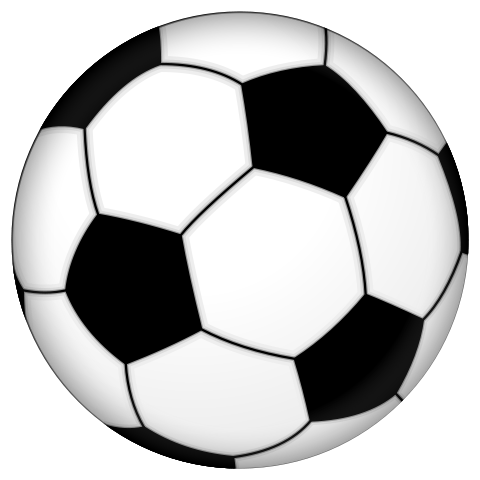
\includegraphics[scale=0.3]{img/Soccer-ball.eps}
 \captionsetup{labelformat=empty}
 \caption{对称群$S_5$是交错群$A_5$与二阶循环群的积。可以描述一个足球的对称}
 \label{fig:S5}
%\end{wrapfigure}
\end{figure}

这样我们就证明了一般5次方程是不能用根式解的。我们也可以从另一个角度做出解释。对称群$S_5$有120个元素,它的唯一正规子群是$A_5$,其中$A_5$叫做交错群,有60个元素。$A_5$的唯一正规子群是$\{1\}$。这一子群链是$S_5 \supset A_5 \supset \{1\}$。但是商群$A_5/\{1\}$不是阿贝尔群(不可交换)。因此它不是可解群。这样它对应的一般5次方程不是根式可解的。

一般4次方程,对称群$S_4$的正规子群是$A_4$,交错群$A_4$有一个正规子群

\[
\{(1), (1 2)(3 4), (1 3)(2 4), (1 4)(2 3)\}
\]

而这个群和克莱因群同构,所以是可解的。

对于三次方程,对称群$S_3$的正规子群$A_3$,交错群$A_3$同构于3阶循环群。所以也是可解的。

\begin{figure}[htbp]
  \centering
  \subcaptionbox{交错群$A_3$相当于3阶循环群}[0.3\linewidth]{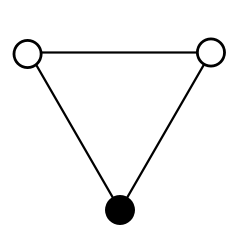
\includegraphics[scale=0.25]{img/C3.eps}} \quad
  \subcaptionbox{对称群$S_3$,其上部为$A_3$}[0.3\linewidth]{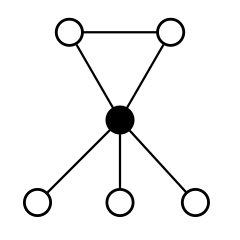
\includegraphics[scale=0.25]{img/S3.eps}}
  \subcaptionbox{交错群$A_4$}[0.3\linewidth]{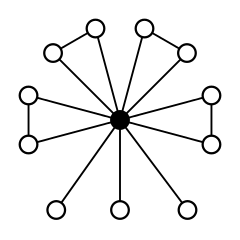
\includegraphics[scale=0.25]{img/A4.eps}}
  \caption{对称群和交错群,黑点是单位元,循环用闭环表示}
  \label{fig:group-graph}
\end{figure}

至此我们简单介绍了伽罗瓦理论。伽罗瓦理论是抽象代数中的强大工具,它可以解决很多问题,如证明代数基本定理、证明当年高斯用尺规作图画出的正17边形是可行的。证明无法用尺规作图完成古希腊三大作图问题——圆化方、三分角、倍立方等等。我们希望读者能通过这一章,领略到抽象思维的深邃和优美。

\begin{Exercise}
\Question{考虑5次方程$x^5 - 1 = 0$,它是根式可解的。它的伽罗瓦群和对应的子群链是什么?}
\end{Exercise}

\section{扩展阅读}

对于抽象代数的基本概念,张禾瑞先生的《近世代数基础》\cite{ZhangHeRui1978}是本入门的教材。这本书不到200页,提纲挈领地减少了群、环、域的基本概念。阿姆斯特朗的《群与对称》\cite{Armstrong1988}同样也是小薄本,对于对称性的讲解是其特色。迈克尔$\cdot$阿廷的《代数》是一本广泛使用的教材,最后一章讲解了伽罗瓦理论。爱德华兹的《伽罗瓦理论》,以历史的发展为主要脉络,用古典的方法来讲述。并且还把伽罗瓦手稿的英文译文置于附录,使读者能了解当初是怎样一步一步解决的问题。章璞先生的《伽罗瓦理论:天才的激情》\cite{ZhangPu2013}则用现代的方法讲解伽罗瓦理论。埃米尔$\cdot$阿廷的《伽罗瓦理论》是这个领域中的经典,有李同孚先生翻译的中译本。韩雪涛的《好的数学》系列中有很多数学家的传记故事,生动有趣。

\ifx\wholebook\relax \else
\begin{thebibliography}{99}

\bibitem{HanXueTao16}
{\fontspec{\cnmainft}韩雪涛 ``数学悖论与三次数学危机''. 人民邮电出版社.} 2016, ISBN: 9787115430434

\bibitem{LiuXinyu2017}
{\fontspec{\cnmainft}刘新宇 ``算法新解'' 人民邮电出版社.} 2017, ISBN: 9787115440358

\bibitem{HanXueTao2009}
{\fontspec{\cnmainft}韩雪涛 ``好的数学——“下金蛋”的数学问题''. 湖南科学技术出版社.} 2009, ISBN: 9787535756725

\bibitem{HanXueTao2012}
{\fontspec{\cnmainft}韩雪涛 ``好的数学——方程的故事''. 湖南科学技术出版社.} 2012, ISBN: 9787535770066

\bibitem{Wiki-Galois-theory}
Wikipedia ``Galois theory''. \url{https://en.wikipedia.org/wiki/Galois_theory}

\bibitem{Wiki-Galois}
Wikipedia ``Évariste Galois''. \url{https://en.wikipedia.org/wiki/Évariste_Galois}

\bibitem{Galois-1832}
Anita R Singh. ``The Last Mathematical Testament of Galois'' Resonance Oct 1999. pp93-100.

\bibitem{Liouville-1846}
Sawilowsky, Shlomo S. and Cuzzocrea, John L. (2005) ``Joseph Liouville’s `Mathematical Works Of Évariste Galois','' Journal of Modern Applied Statistical Methods: Vol. 5 : Iss. 2 , Article 32. DOI: 10.22237/jmasm/1162355460

\bibitem{StepanovRose15}
Alexander A. Stepanov, Daniel E. Rose ``From Mathematics to Generic Programming''. Addison-Wesley Professional; 1 edition (November 17, 2014) ISBN-13: 978-0321942043

\bibitem{Wiki-Rubik-Cube-group}
Wikipedia ``魔方群''. \url{https://en.wikipedia.org/wiki/Rubik's_Cube_group}

\bibitem{ZhangHeRui1978}
张禾瑞 ``近世代数基础''. 高等教育出版社. 1978, ISBN: 9787040012224

\bibitem{Armstrong1988}
M.A. Armstrong ``群与对称(影印版)''. Springer. 1988. ISBN: 0387966757.

\bibitem{Wiki-Lagrange}
Wikipedia ``约瑟夫$\cdot$拉格朗日''. \url{https://en.wikipedia.org/wiki/Joseph-Louis_Lagrange}

\bibitem{Wiki-FLT-proof}
Wikipedia ``费马小定理的证明''. \url{https://en.wikipedia.org/wiki/Proofs_of_Fermat's_little_theorem}

\bibitem{Wiki-Euler}
Wikipedia ``莱昂哈德$\cdot$欧拉''. \url{https://en.wikipedia.org/wiki/Leonhard_Euler}

\bibitem{Wiki-Carmichael-number}
Wikipedia ``卡米歇尔数''. \url{https://en.wikipedia.org/wiki/Carmichael_number}

\bibitem{Algorithms-DPV}
Sanjoy Dsgupta, Christos Papadimitriou, Umesh Vazirani. 钱枫 邹恒明 注释. ``算法概论(注释版)''. 机械工业出版社. 2009年1月. ISBN: 9787111253617

\bibitem{Wiki-Miller-Rabin}
Wikipedia ``米勒——拉宾素数检验''. \url{https://en.wikipedia.org/wiki/Miller-Rabin_primality_test}

\bibitem{Wiki-Noether}
Wikipedia ``埃米$\cdot$诺特''. \url{https://en.wikipedia.org/wiki/Emmy_Noether}

\bibitem{ZhangPu2013}
章璞. ``伽罗瓦理论:天才的激情''. 高等教育出版社. 2013年5月. ISBN: 9787040372526

\bibitem{Stillwell1994}
John Stillwell. ``Galois Theory for Beginners''. The American Mathematical Monthly, Vol. 101, No. 1 (Jan., 1994), pp. 22-2

\bibitem{Goodman2011}
Dan Goodman. ``An Introduction to Galois Theory''. \url{https://nrich.maths.org/1422}

\bibitem{MArtin}
Michael Artin. ``代数(英文版,第二版)''. 机械工业出版社. 2011年12月. ISBN: 9787111367017

\end{thebibliography}

\expandafter\enddocument
%\end{document}

\fi
